%% Version 4.3.2, 25 August 2014
%
%%%%%%%%%%%%%%%%%%%%%%%%%%%%%%%%%%%%%%%%%%%%%%%%%%%%%%%%%%%%%%%%%%%%%%
% Template.tex --  LaTeX-based template for submissions to the 
% American Meteorological Society
%
% Template developed by Amy Hendrickson, 2013, TeXnology Inc., 
% amyh@texnology.com, http://www.texnology.com
% following earlier work by Brian Papa, American Meteorological Society
%
% Email questions to latex@ametsoc.org.
%
%%%%%%%%%%%%%%%%%%%%%%%%%%%%%%%%%%%%%%%%%%%%%%%%%%%%%%%%%%%%%%%%%%%%%
% PREAMBLE
%%%%%%%%%%%%%%%%%%%%%%%%%%%%%%%%%%%%%%%%%%%%%%%%%%%%%%%%%%%%%%%%%%%%%

%% Start with one of the following:
% DOUBLE-SPACED VERSION FOR SUBMISSION TO THE AMS
\documentclass{ametsoc}

% TWO-COLUMN JOURNAL PAGE LAYOUT---FOR AUTHOR USE ONLY
% \documentclass[twocol]{ametsoc}

%%%%%%%%%%%%%%%%%%%%%%%%%%%%%%%%
%%% To be entered only if twocol option is used

\journal{jcli}

%  Please choose a journal abbreviation to use above from the following list:
% 
%   jamc     (Journal of Applied Meteorology and Climatology)
%   jtech     (Journal of Atmospheric and Oceanic Technology)
%   jhm      (Journal of Hydrometeorology)
%   jpo     (Journal of Physical Oceanography)
%   jas      (Journal of Atmospheric Sciences)	
%   jcli      (Journal of Climate)
%   mwr      (Monthly Weather Review)
%   wcas      (Weather, Climate, and Society)
%   waf       (Weather and Forecasting)
%   bams (Bulletin of the American Meteorological Society)
%   ei    (Earth Interactions)

%%%%%%%%%%%%%%%%%%%%%%%%%%%%%%%%
%Citations should be of the form ``author year''  not ``author, year''
\bibpunct{(}{)}{;}{a}{}{,}

%%%%%%%%%%%%%%%%%%%%%%%%%%%%%%%%

%%% To be entered by author:

%% May use \\ to break lines in title:

\title{The Rainband Detection Algorithm (RDA): Frontal Rainfall in China. Part I: Climatology}

%%% Enter authors' names, as you see in this example:
%%% Use \correspondingauthor{} and \thanks{Current Affiliation:...}
%%% immediately following the appropriate author.
%%%
%%% Note that the \correspondingauthor{} command is NECESSARY.
%%% The \thanks{} commands are OPTIONAL.

    %\authors{Author One\correspondingauthor{Author One, 
    % American Meteorological Society, 
    % 45 Beacon St., Boston, MA 02108.}
% and Author Two\thanks{Current affiliation: American Meteorological Society, 
    % 45 Beacon St., Boston, MA 02108.}}

\authors{Jesse A. Day\correspondingauthor{Jesse Day, University of California, Department of Earth and Planetary Science, College of Letters and Science, 307 McCone Hall, Berkeley, CA 94720.}, Inez Y. Fung and Weihan Liu}

%% Follow this form:
    % \affiliation{American Meteorological Society, 
    % Boston, Massachusetts.}

\affiliation{Department of Earth and Planetary Science, University of California Berkeley, Berkeley, California}

%% Follow this form:
    %\email{latex@ametsoc.org}

\email{jessed@berkeley.edu}

%% If appropriate, add additional authors, different affiliations:
    %\extraauthor{Extra Author}
    %\extraaffil{Affiliation, City, State/Province, Country}

%\extraauthor{}
%\extraaffil{}

%% May repeat for a additional authors/affiliations:

%\extraauthor{}
%\extraaffil{}

%%%%%%%%%%%%%%%%%%%%%%%%%%%%%%%%%%%%%%%%%%%%%%%%%%%%%%%%%%%%%%%%%%%%%
% ABSTRACT
%
% Enter your abstract here
% Abstracts should not exceed 250 words in length!
%
% For BAMS authors only: If your article requires a Capsule Summary, please place the capsule text at the end of your abstract
% and identify it as the capsule. Example: This is the end of the abstract. (Capsule Summary) This is the capsule summary. 

\abstract{The topography and land-sea contrast of East Asia favor year-round frontal storm tracks extending thousands of miles. We create a recursive image processing algorithm, the Rainband Detection Algorithm (RDA), that detects rainbands in maps of daily rainfall and quantifies their attributes. By applying RDA to the APHRODITE database of Asian monsoon rainfall, we produce a 57-year (1951-2007) daily catalog of rainband occurrences over China. Our catalog quantifies the seasonal progression of the East Asian monsoon and Meiyu Front in unprecedented fashion.
\begin{document}

%% Necessary!
\maketitle


%%%%%%%%%%%%%%%%%%%%%%%%%%%%%%%%%%%%%%%%%%%%%%%%%%%%%%%%%%%%%%%%%%%%%
% MAIN BODY OF PAPER
%%%%%%%%%%%%%%%%%%%%%%%%%%%%%%%%%%%%%%%%%%%%%%%%%%%%%%%%%%%%%%%%%%%%%
%

%% In all cases, if there is only one entry of this type within
%% the higher level heading, use the star form: 
%%
% \section{Section title}
% \subsection*{subsection}
% text...
% \section{Section title}

%vs

% \section{Section title}
% \subsection{subsection one}
% text...
% \subsection{subsection two}
% \section{Section title}

%%%
% \section{First primary heading}

% \subsection{First secondary heading}

% \subsubsection{First tertiary heading}

% \paragraph{First quaternary heading}


\section{Introduction} 

 	Eastern China receives about 60\% of its precipitation from May to August via the East Asian summer monsoon. The period of peak rainfall lasting from early June to mid-July is called ``Meiyu season'' (lit. ``plum rains,'' referring to the spectacular growth of plum blossoms in central China with the onset of heavy rains). During this time, heavy rainfall occurs in zonal bands resulting from frontal synoptic conditions (the ``Meiyu front''). The rainfall climatology of Japan and Korea also features similar phenomena, known as Baiu and Changma respectively, that deliver key fractions of total yearly rainfall. A growing volume of evidence suggests a shift in rainfall over China beginning in the late 1970s, featuring a ``South Flood-North Drought'' pattern shown in Figure~\ref{fig:f31} \citep{Hu1997,Gong2002,Nigam2013}.  A permanent change would have major humanitarian impacts on densely-populated eastern China, where a sizable fraction of the population depends on agriculture for subsistence. Northern China already suffers from substantial depletion of freshwater resources along with increasing demand \citep{Currell2012,Gleeson2012}. The Chinese government has embarked on a project to reroute water from the Yangtze River to northern China, the South-North Water Transfer Project (\textit{nanshui beidiao gongcheng}), which is expected to become the most expensive hydraulic engineering project ever undertaken and will entail massive human and environmental impact \citep{Magee2011}. Under such circumstances, it is vital to understand whether this pattern will strengthen under global warming, or represents only a temporary deviation from the mean. 
	
	The climatology of the East Asian monsoon is unique when compared to other monsoon circulations \citep{Ding2005}. Whereas understanding of tropical monsoons has progressed greatly via theoretical studies \citep{Plumb1992,Prive2007,Bordoni2008}, the dynamics that favor the existence of frontal convection over East Asia in summer remain a point of debate, centering around the interplay of the tropospheric jet and Tibetan Plateau \citep{Molnar2010,Sampe2010,Chen2014}. Therefore, no simple conceptual template exists for interpreting the South Flood-North Drought. However, it is known that the migration of the Meiyu front entails a series of large-scale circulation changes \citep{Chen2004}, and furthermore that anomalies in Meiyu front latitude produce corresponding rainfall anomalies \citep{Kosaka2011}. Therefore, the South Flood-North Drought should be describable in terms of changes in the mean properties of Meiyu rainbands, such as a shift in latitude, a change in intensity, or an earlier or delayed northward migration. In turn, such a characterization may elucidate the dynamics responsible for the change.
	
	We have developed a recursive fitting algorithm, the Rainband Detection Algorithm (RDA), that locates frontal rainbands in a daily precipitation map and quantifies their attributes. Using the APHRODITE rain gauge product, we have created a 57-year (1951-2007) daily database of rainband attributes in China. Previous studies have investigated the statistics of the Meiyu front on decadal and even centennial timescales \citep{Chen2004,Ge2008,Xu2009}, but to our knowledge no previous author has compiled a multi-decadal daily catalog of events. We use this catalog to find the late \nth{20}-century changes in rainband statistics that have caused the South Flood-North Drought. Furthermore, since rainbands are produced by frontal atmospheric conditions, late \nth{20}-century changes in rainband attributes may reflect corresponding changes in East Asian monsoon dynamics, and ultimately be influenced by \nth{20}-century warming. We propose an altered progression of the tropospheric jet as proximal cause in the conclusion, and elaborate on this theory in Chapter 4.
		
\section{APHRODITE}

	The APHRO\_MA\_V1101 product from APHRODITE (Asian Precipitation - Highly-Resolved Observational Data Integration Towards Evaluation of the Water Resources) includes 57 years (1951-2007) of daily rainfall (PRECIP product) on a .25$^{\circ} \times .25^{\circ}$ grid over 60$^{\circ}$-150$^{\circ}$E and 15$^{\circ}$S-55$^{\circ}$N \citep{Yatagai2012}. Values are assimilated from weather station observations and therefore available over land only. We focus on the subregion inside of 100$^{\circ}$E-123$^{\circ}$E and 20$^{\circ}$N-40$^{\circ}$N, where Meiyu rainbands occur. Stations in this region are spaced at 100-200 km intervals (shown by RSTN product), such that rainbands are clearly resolved. APHRODITE's resolution cannot capture some features visible in TRMM satellite data \citet{Xu2009}, but its length allows for the study of decadal change. Since almost all precipitation in this region falls as rain, we use the words ``rainfall'' and ``precipitation'' interchangeably in the rest of this work.
	
\section{Rainband Detection Algorithm (RDA)}

\subsection{Overview}

	For each day from 1 January 1951 to 31 December 2007 (20,819 days total), RDA determines whether a rainband exists inside the window of 105-123$^{\circ}$E and 20-40$^{\circ}$N, a region hereafter referred to as ``East China.'' A rainband is defined as a continuous chain of rainfall maxima exceeding 10 mm day$^{-1}$ spanning at least 5$^{\circ}$ of longitude. If a rainband exists, its properties are calculated including latitude, intensity, tilt, length and width, as well as a ``quality score'' $Q$, defined as the fraction of daily total East China rainfall falling within the band. Fits with poor $Q$ are discarded. We also test for the existence of two rainbands on a single day, an arrangement commonly found in August and September. In such a case, the first and second fitted rainbands are referred to as ``primary'' and ``secondary'' rainbands respectively. A description of algorithm functionality in greater detail follows.
	
	We cannot distinguish between the mechanisms that supply rainfall. Any storm that propagates zonally over the course of a day will be interpreted as a rainband, regardless even of whether it propagates westward or eastward. However, from observation, storms reaching East China during the rainiest months of the East Asian summer monsoon are predominantly westerly \citep{Day2015}. Therefore, we expect that RDA detects similar types of rainfall events from one summer to the next, allowing for meaningful analysis of decadal changes.  
	
\subsection{Recursive Convergent Image Processing}

\begin{enumerate}
	\item Given a daily map of East China rainfall (105-123$^{\circ}$E, 20-40$^{\circ}$N) at $.25^{\circ} \times .25^{\circ}$ resolution, the maximum rainfall intensity $int_{max}$ and its latitude $lat_{max}$ are recorded at each longitude. If there exists a continuous chain of maxima spanning $5^{\circ}$ of longitude (20 points in a row) where $int_{max}$ exceeds 10 mm day$^{-1}$, we proceed to step 2 and attempt a rainband fit (Figure~\ref{fig:f32}a). Otherwise, there is no rainband and no fit is attempted for that day (Figure~\ref{fig:f32}b).
	
	\item A weighted least-squares linear regression of $lat_{max}$ using $int_{max}$ as weighting approximates the position of the rainband with a straight line (a reasonable assumption from observation). To encourage convergence, the weight of outlying maxima is set to zero. An outlier is defined as any maximum where $lat_{max}$ is over $5^{\circ}$ of latitude away from  $\left<lat_{max}\right>$, the centroid of $lat_{max}$ weighted by $int_{max}$\footnote{In rare cases with two rainbands of roughly equal strength that are well-separated in latitude, the centroid of precipitation may lie midway between the bands such that all maxima will be thrown out as outliers. To avoid this scenario, we verify after removing outliers that

%% FOOTNOTE
	\begin{equation*}
	 \sum\limits_{long} weights > 200 \mathrm{\ mm\ day}^{-1}
	\end{equation*}
	
 	When this condition is failed, which can only occur when too many of our maxima have been discarded, we return to step 1 and find maxima inside a subwindow with latitude range of 20$^{\circ}$N-$\left<lat_{max}\right>$ or $\left<lat_{max}\right>$-40$^{\circ}$N, depending on which half of our domain has a longer chain of maxima exceeding 10 mm day$^{-1}$. The remaining steps of our algorithm are applied as usual. The search for a secondary rainband and calculation of quality scores are performed over the whole East China window (20$^{\circ}$N-40$^{\circ}$N).}, calculated as %%END FOOTNOTE

	\begin{equation*}
	\left<lat_{max}\right>=\frac{\sum_{long} lat_{max}*int_{max}}{\sum_{long} \max}
	\end{equation*}

	\item A recursive algorithm converges from this initial fit to a best estimate of rainband position. In each iteration, we find a new set of maxima within \textit{k} degrees of the previous best fit line, and again perform a weighted linear fit of the maxima (Figure~\ref{fig:f33}a). $k$ is progressively decreased with each iteration from $5^{\circ}$ to $2^{\circ}$ by $.25^{\circ}$ increments, and then from $2^{\circ}$ to $.25^{\circ}$ by $.25^{\circ}$ increments repeating each width $k$ twice in a row (Figures~\ref{fig:f33}b-c). The fit obtained in the final iteration is taken as our best estimate (Figure~\ref{fig:f33}d).
	
	\item We define the ``quality score'' $Q$ as the fraction of daily total East China rainfall (the sum of all rainfall inside of 105-123$^{\circ}$E and 20-40$^{\circ}$N) that falls within $2.5^{\circ}$ degrees of the best estimate line (Figure~\ref{fig:f34}b). Other rainband properties are calculated as follows:
	
	 \begin{enumerate}
	 
	 	\item \textit{Latitude}: The latitude of the best fit line at 115$^{\circ}$E. 
	 
	 	\item \textit{Intensity}: Mean rainfall of all ``rainband points'' (points along the best fit line where daily rainfall exceeds 5 mm day$^{-1}$).
	 
	 	\item \textit{Length}: Total number of rainband points (units of degrees longitude)
	 
	 	\item \textit{Width}: Mean distance between half-maxima ($int_{max}$/2) on either side of each rainband point (units of degrees latitude).
	 
	 \end{enumerate}
	
	\item After finding a primary rainband, we check for the existence of a secondary rainband by removing all \textit{banded rainfall} associated with the primary band from the daily rainfall map. \textit{Banded rainfall} is defined as all rainfall falling within 4$^{\circ}$ of a rainband axis and any other adjacent points where rainfall exceeds 10 mm day$^{-1}$ (see Figure~\ref{fig:f35}a for an example). After removing primary rainband rainfall, we reapply the continuous maximum criterion from step 1 (Figure~\ref{fig:f35}b). If passed, steps 2-4 are repeated to find a best estimate for the position of the secondary rainband, and its attributes calculated.
	
	\item If a secondary rainband is found, two additional \textit{conditional} quality scores $Q_1$ and $Q_2$ are calculated. $Q_1$ is the fraction of total daily East China rainfall that fell within $2.5^{\circ}$ degrees of the primary rainband \textit{after removing all rainfall associated with the secondary rainband} (effectively the $Q$ score if the secondary rainband didn't exist). Likewise, $Q_2$ is the $Q$ score of the second rainband \textit{after removing all rainfall from the primary rainband}. An example is shown in Figure~\ref{fig:f34}d.		
	
\end{enumerate} 

\subsection{Quality Control}

	After running the algorithm for all 20,819 days from 1 January 1951 to 31 December 2007, we obtained 11,228 days with at least one rainband and 1,116 days with two rainbands. Subsequently, we apply a quality control (QC) algorithm to eliminate days with poor fit, based on the quality scores $Q$, $Q_1$ and $Q_2$ as well as the ``Taiwan fraction'' $TW$, defined as the percentage of daily total East China rainfall falling over the island of Taiwan (roughly 120-$122^{\circ}$E and 22-$26^{\circ}$N). Rainband fits are deemed successful if they satisfy the following two criteria:

\begin{enumerate}

	\item $TW < 20\%$. If $TW > 20\%$, the day's fit is thrown out (238 cases total, 2.1\% of total fits). Such days are dominated by tropical storms reaching Taiwan and do not exhibit a strong rainband (example shown in Figure~\ref{fig:f34}a).  
	
	\item The quality scores of the fit must meet either of the two following benchmarks:
	
	\begin{enumerate} 
	
	\item If $Q>.6$, the fit is deemed successful (7,522 days, 67.0\% of total fits; Figure~\ref{fig:f34}b). If $Q_2$ is also greater than .6, the day will be classified as a double rainband day (Type I double rainband; 232 cases). 3.1\% of days where $Q>.6$ also achieve $Q_2>.6$.
		
	\item If $Q<.6$, the fit is discarded unless two rainbands are detected and both $Q_1 > .6\mathrm{\ \textbf{and}\ }Q_2 > .6$ (where again $Q_1$ and $Q_2$ are \textit{conditional} quality scores as defined above). In such cases, the presence of multiple rainbands of similar intensity initially obscures the goodness of fit (Figure~\ref{fig:f34}d). Such days are also classified as double rainband days (Type II double rainband; 466 cases).
	
	\end{enumerate}
	
	If neither criterion 2a nor 2b is satisfied, the fit is thrown out (Figure~\ref{fig:f34}c).
	
\end{enumerate}	

	The use of conditional quality scores $Q_1$ and $Q_2$ adds 466 double rainband fits (6.2\% of all successful fits) that would otherwise have been missed due to $Q<.6$. 33.2\% of double rainband days are Type I ($Q>.6$) and 66.8\% Type II ($Q<.6$) as defined above. Double rainbands are more common during certain months, particularly July-September. Tables~\ref{tab:t31}-~\ref{tab:t33} contain detailed results of the application of RDA to years 1951-2007 in APHRODITE. The entire catalog is publicly available on the author's website.

\subsection{Rainfall Types}
	
	RDA allows us to classify all rainfall on each day as either \textit{banded} (falls within a rainband) or \textit{local}. \textit{Banded} rainfall consists of all rainfall falling within 4$^{\circ}$ of a rainband axis and any other adjacent points where rainfall exceeds 10 mm day$^{-1}$, the same definition as in step 5 of the recursive algorithm above. An example is shown in Figure~\ref{fig:f35}a. Rainfall on each of the 20,819 available days was partitioned into its banded and local components. This allows us to determine what fraction of rainfall at each point in East China is supplied via banded rainfall (Figure~\ref{fig:frontpct}). We also test for the significance of decadal changes in banded and local rainfall separately (Figure~\ref{fig:decadal_front}). These results are discussed below. Videos of the climatological progression of banded and local rainfall are available at the author's website and on request, as well as daily maps of banded and local rainfall for the years 1951-2007.
	
\section{Methods}	

\subsection{Alternative Metrics of China Rainfall}

Since the RDA method is complex, we must justify its use by proving that it supplies information about China rainfall beyond what simpler metrics can provide. We define a suite of potential daily rainfall metrics as follows: 

\begin{itemize}

	\item $M_1$ - Latitude of maximum rainfall;
	
	\item $M_2$ - Intensity-weighted centroid of daily rainfall latitude;
	
	\item $M_3$ - Intensity of maximum rainfall over China (100-123$^{\circ}$E and 20-40$^{\circ}$N);
	
	\item $M_4$ - Area-averaged intensity of China rainfall; 
	
	\item $M_5$ - Area-averaged intensity of North China rainfall (107.5-125$^{\circ}$E and 37-42$^{\circ}$N); 
	
	\item $M_6$ - Area-averaged intensity of South China rainfall (107.5-122.5$^{\circ}$E and 27-33$^{\circ}$N); 
	
	\item $M_7$ - \% of days where $M_5$ exceeds 1 mm day$^{-1}$ (\textit{frequency} of North China rainfall);
	
	\item $M_8$ - \% of days where $M_6$ exceeds 1 mm day$^{-1}$ (\textit{frequency} of South China rainfall).
	
\end{itemize}

 The definitions of the North China and South China regions are the same as in \citet{Yu2010}. Each metric is subjected to the same tests of significance applied to changes in rainband behavior between time periods. The climatologies of $M_1-M_8$ are shown in Figure~\ref{fig:type_changes}a-d, and mean values during different seasons listed in Tables~\ref{tab:t39}-\ref{tab:t311}. The significance of changes in each metric between 1951-1979 and 1980-2007 is displayed in Table~\ref{tab:t312}. Section 3.6 discusses results.

\subsection{Temporal Autocorrelation}

	Fronts and rainbands tend to persist for several days. Therefore, rainfall amounts and front attributes on successive days are not fully independent observations, which reduces the effective number of degrees of freedom of these time series. This temporal autocorrelation must be accounted for in calculations of statistical significance such as estimating the $p$-value of a change in rainband frequency between two time periods. In this particular case, we use the analytic formula for a Bernoulli process (applicable for any time series where observations are binary) with effective number of degrees of freedom $n=\frac{N}{\tau}$ for number of days $N$ and decorrelation time $\tau$ given by

\begin{equation*}
\tau=1+2\sum_{k=1}^m \rho(k)
\end{equation*}

	where $\rho(k)$ is the autocorrelation function of rainband existence with lag $k$ \citep{VonStorch1999}. We calculate $\tau$ using a maximum lag of $m=10$ days. The yearly mean decorrelation timescale of rainband frequency is found to be $\tau = 1.81$ after removing the seasonal cycle. This value is used to calculate significance of changes in Figure 3b. The standard deviation and $p$-values of rainband frequency changes in Tables~\ref{tab:t35} and~\ref{tab:t37} use seasonal values of $\tau$ calculated in \ref{tab:t34}. Similarly, Table~\ref{tab:t311} shows the $\tau$ of alternative metrics of China rainfall, which is then used to calculate the significance of decadal changes in Table~\ref{tab:t312}. $\tau$ is also used to select block length for moving blocks bootstrap tests, as described below.

%% BOOTSTRAPPING
\subsection{Significance of Changes: Bootstrapping Algorithms}

	Observations of rainband latitude and intensity during a given time period obey unknown distributions. Therefore, we require non-parametric tests to estimate the standard deviation of their mean and the significance of changes in mean. We employ bootstrapping with and without replacement (the latter also known as a permutation test), well-established techniques that estimate quantities of interest by constructing synthetic distributions with random sampling of original data \citep{Good2005}. We use bootstrapping with replacement to calculate the standard deviation of means (Tables~\ref{tab:t34},~\ref{tab:t36} and~\ref{tab:t38}). We focus on changes in front attributes between 1951-1979 and 1980-2007 (Tables~\ref{tab:t35} and~\ref{tab:t36}), and also repeat our methodology for 1979-1993 versus 1994-2007 (Tables~\ref{tab:t37} and~\ref{tab:t38}). $p$-values listed are from permutation testing with 10,000 iterations; the results of bootstrapping with and without replacement are very similar.
	
	The bootstrap must be adapted for time series featuring temporal autocorrelation. In such time series, a single anomalous weather event will persist over several days, and a bootstrap method will tend to exaggerate the significance of differences between the two original distributions. To avoid this scenario, we use a \textit{moving blocks bootstrap} test, described for instance in \citet{Singh2014}. This technique is identical to bootstrapping with replacement except that samples are drawn in continuous blocks of length $n$ that preserve the time structure of the original data set. Block length is chosen based on decorrelation time scale $\tau$. The autocorrelation of daily rainfall in China is $\tau =\mytilde 3$ days, and therefore the significance estimates in Figure~\ref{fig:hov}a use a moving blocks bootstrap with block length of 3 days and 1000 iterations. The calculation of significance of change in alternative China rainfall statistics $M_1-M_6$ (Table~\ref{tab:t312}) uses the $\tau$ of each statistic in each season (Table~\ref{tab:t311}) rounded to the nearest integer as block length. In general, a choice of block lengths between 2 and 5 days leads to similar results. Our MATLAB code for the permutation test and the moving blocks bootstrap is included in the appendix.
	
	The moving blocks bootstrap cannot be used for time series with gaps. Therefore, we use a permutation test to estimate the significance of changes in mean latitude and intensity of rainbands between time periods (Tables~\ref{tab:t36} and~\ref{tab:t38}). These latter results are verified with Anderson-Darling and Kolmogorov-Smirnov tests, two methods which estimate the significance of shifts in distribution between two sample. These tests are described below.

\subsection{Significance of Changes in Distribution}

In addition to gauging the significance of changes in mean, we can also test the probability that two samples were drawn from the same distribution. The Kolmogorov-Smirnov and Anderson-Darling tests each define a test statistic based on the largest difference between the observed probability distribution of two samples. Similar to a $t$-test, the value of this test statistic can be translated into a $p$-value. We first define the \textit{empirical distribution function} $F_1(x)$ and $F_2(x)$ of each sample. All $n$ observations in each sample are ordered as $\left\{X_1 < ... < X_n\right\}$, after which $F(x)$ is calculated as follows:

\begin{align}
	F(x) =& \frac{1}{n}\sum_{i=1}^n I_{[-\infty,x]} (X_i) \\
	I_{[-\infty,x]} =& 
	\begin{cases}
   		 1 & \text{if } X_i \leq x\\
    		0 & \text{otherwise} \\
    	\end{cases}
\end{align}

 The K-S test statistic $D$ is then defined as the maximal distance between the two empirical distribution functions:

\begin{equation}
	D=\max_{all\ x} |F_{1}(x)-F_{2}(x)|
\end{equation}

$D$ can then be inverted to derive a $p$-value. The Anderson-Darling (A-D) test statistic $A^2$ resembles $D$, but is formulated to be more sensitive to the tails of the distribution:

\begin{equation}
	A^2 = -n-S \,,
	\mathrm{where}
\end{equation}

\begin{equation}
	S=\sum_{i=1}^n \frac{2i-1}{n}\left[\ln(F(X_i)) + \ln\left(1-F(X_{n+1-i})\right)\right].
\end{equation}

$A^2$ can likewise be translated into a $p$-value. The K-S and A-D tests cannot be used if values are repeated within samples, because $D$ and $A^2$ are then undefined. We solve this problem by using bootstrap versions of these tests. Bootstrap K-S and A-D tests were performed using the programming language R with 10,000 iterations. The significance of changes in the distribution of rainband latitude and intensity are presented in Tables~\ref{tab:t313} and~\ref{tab:t314}. Both tests produce fairly similar results.

\section{Results}

\subsection{Rainband Climatology}

	We compile our daily rainband catalog into a 57-year daily climatology (1951-2007). The yearly progression of precipitation over eastern China is shown in Figure~\ref{fig:hov}a, longitudinally averaged over $100-123^\circ$E with a 5-day running mean, similar to Figure 7 in \citet{Ding2005}. China receives a substantial fraction of its yearly precipitation outside of summer, unlike other monsoonal regions which tend to be very dry in winter \citep{Wang2002}. Figure~\ref{fig:hov}b shows a Hovm\"oller diagram of the probability of rainband occurrence at each latitude, including both primary and secondary rainbands. Some periods of heavy rainfall, in particular the August peak over southern China (over 10 mm day$^{-1}$ around 20$^{\circ}$N), do not correspond to a surge in rainband frequency. Figure~\ref{fig:hov}c shows the probability of rainband occurrence and mean intensity on each day. Figure~\ref{fig:hov}d shows mean rainband tilt and length, as well as the conditional probability of observing a secondary rainband given the presence of a primary rainband. Frontal rainbands over China can appear in any month, with their probability of occurrence and intensity maximizing in late June (80\% probability of occurrence, mean intensity of 31 mm day$^{-1}$) and minimizing in January (10\% probability occurrence, mean intensity of 12 mm day$^{-1}$).
	
	Abrupt climatological shifts occur simultaneously in both rainfall and rainband climatology. We define 5 periods of distinct behavior as demarcated in Figure~\ref{fig:hov}: 

\begin{enumerate}

\item The Spring Rains (days 60-120, March 1-April 30), previously studied in \citet{Tian1998}, marked by frequent but relatively weak rainbands (47\% occurrence, 20 mm day$^{-1}$ mean);

\item Pre-Meiyu season (days 121-160, May 1-June 9), during which rainfall and front intensity steadily increase (56\% occurrence, 25.5 mm day$^{-1}$ mean);

\item Meiyu season (days 161-200, June 10-July 19) when a remarkable 7-degree northward shift in mean rainband latitude occurs over the course of several weeks, and rainband frequency and intensity peaks (66\% occurrence, 28.3 mm day$^{-1}$ mean); 

\item Post-Meiyu season (days 201-273, July 20-September 30), when rainbands are less common than during the Spring Rains (42\% occurrence) but double rainbands occur more frequently (28\% chance of observing a secondary rainband if a primary rainband is observed); 

\item The Fall Rains (days 274-320, October 1-November 16), when mean rainband latitude shifts back southward from its northern maximum of 30$^\circ$N and rainband frequency decreases to just 27\%. 

\end{enumerate}

	The Pre-Meiyu, Meiyu and Post-Meiyu are equivalent to the three stages of Meiyu rainfall described in \citet{Ding2005}. The transition from Pre-Meiyu to Meiyu and from Meiyu to Post-Meiyu both entail striking, sudden changes in rainband behavior. The onset of the Meiyu is marked by a climatological jump in rainband frequency and intensity around day 160 (June 9) that persists for 20 days when rainbands are concentrated between 26$^\circ$ and 30$^\circ$N. Yet by day 200 (July 19), this same region is less likely than any other latitude to feature a rainband, roughly an 80\% local decline in frequency in the span of 3 weeks (Figure~\ref{fig:hov}b). Rainbands are generally more probable and stronger during spring than in fall, and the intensification of rainband activity during the Meiyu and abrupt northward jump have no counterpart in the Fall Rains. The causes of this seasonal asymmetry merit further study.
	
	These results can be compared with the frontal event catalog of \citet{Xu2009}, which finds a similar date for the northward transition of the Meiyu front. The total number of rainband counts as well as the mean and standard deviation of rainband frequency, latitude and intensity during each time period are presented in Table~\ref{tab:t34}. Figure~\ref{fig:frontpct} shows that frontal rainfall constitutes at least 40\% of yearly total for all of mainland China east of 105$^\circ$E between 21$^\circ$N and 37$^\circ$N, over 60\% for most of central China, and up to 74\% in the vicinity of Jiangxi Province (28$^\circ$N, 116$^\circ$E). Thus, banded rainfall is an essential component of East China's yearly rainfall budget.
			
\subsection{Rainband Changes}

\subsubsection{1980-2007 versus 1951-1979}

%% NEW PARAGRAPH - SIMPLY DESCRIBES THE YEARLY CUMULATIVE SOUTH FLOOD-NORTH DROUGHT
	The yearly mean change in rainfall rate between 1951-1979 and 1980-2007 over the region 100$^{\circ}$-142$^{\circ}$E and 20$^{\circ}$-48$^{\circ}$N is shown in Figure~\ref{fig:f31}. The South Flood-North Drought refers in particular to a meridional dipole of decadal rainfall change over eastern China (110$^{\circ}$-125$^{\circ}$E and 22$^{\circ}$-42$^{\circ}$N), where most of China's population resides. Pronounced local shifts are also visible in Taiwan, South Korea and parts of Japan. This work focuses on eastern China. Annual changes in northern China between 35$^{\circ}$-40$^{\circ}$N are significant at a 95\% confidence level, whereas changes in central and southern China are not. However, there are substantial changes in central and southern China rainfall during particular Meiyu stages, as shown in Figure~\ref{fig:changes}a and discussed below.
		
	We test whether the rainband catalog reflects the South Flood-North Drought by calculating changes in rainband frequency during 1980-2007 relative to 1951-1979 (shown as a Hovm\"oller diagram in Figure~\ref{fig:changes}b). We also calculate the significance of changes in rainband attributes during each of the five Meiyu stages (Tables~\ref{tab:t35} and~\ref{tab:t36}). During the Pre-Meiyu (days 121-160), the probability of observing a primary rainband has declined from $59.0\% \pm 2.0\%$ to $53.0\% \pm 2.1\%$ ($p=0.020$; Table~\ref{tab:t35}. Figure~\ref{fig:changes} shows matching decreases in front occurrence and rainfall over central China during this time period. The Pre-Meiyu decrease in rainfall was previously reported by \citet{Xin2006}, who linked it to decadal change in the North Atlantic Oscillation (NAO), and also by \citet{Wang2009}. We propose that diminished rainband occurrence has caused this decrease.
		
	In addition, a southward shift in mean rainband latitude has occurred during the Post-Meiyu (days 201-273, or July 20-Sep 30). We focus on rainbands north of 27$^{\circ}$N; rainbands occurring south of this latitude are produced by the westward-propagating remnants of tropical storms, and therefore dynamically unrelated to other storminess during Meiyu season \citep{Day2015}. Considering both primary and secondary rainbands north of 27$^{\circ}$N, mean latitude during 1951-1979 was $33.6^\circ \textrm{N} \pm .3^\circ$ versus $32.9^\circ \textrm{N} \pm .3^\circ$ during 1980-2007 ($p=.0003$; Table~\ref{tab:t36}). This shift remains significant if we do not restrict by front latitude ($p=.0048$). A Post-Meiyu rainfall increase in central China and decrease in northern China has also occurred, producing a South Flood-North Drought pattern (Figure~\ref{fig:changes}c). As a result, yearly rainfall has increased in central China even though Pre-Meiyu rainfall changes in that region are actually negative (Figure~\ref{fig:changes}a). Unlike \citet{Yu2010}, our catalog does not exhibit a \nth{20}-century decrease in the intensity of Yangtze River region frontal rainbands during July-August. A significant southward shift in rainband latitude is also found for the whole year ($p=.0032$, Table~\ref{tab:t36}), but this signal is dominated by the Post-Meiyu shift.
	
	%SHORT PARAGRAPHLET on the 1979-1993 v 1994-2007 jump.
\subsubsection{1979-1993 versus 1994-2007}
	
	We test this methodology also with the set of years 1979-1993 versus 1994-2007, when past authors have reported a shift in South China rainfall \citep{Kwon2007,Wu2010,Yim2013}. The most distinctive change between these two sets of years occurred during Meiyu season, during which rainband latitude shifted southward from $30.0^\circ \textrm{N} \pm .4^\circ$ to $28.9^\circ \textrm{N} \pm .4^\circ\ (p=.0002)$ and the \textit{intensity} of rainbands also jumped from $27.3 \pm 1.1$ mm day$^{-1}$ to $29.8 \pm 1.1$ mm day$^{-1}\ (p=.9994)$, leading to increased rainfall over central and southern China. \citet{Zou2015} also found that China experienced a more intense Meiyu during the 1990s, as well as generally more severe rainfall events. Unlike the comparison between 1951-1979 and 1980-2007, rainband \textit{frequency} remained unchanged. We infer that changes in frequency versus changes in intensity may signal the existence of two different types of external forcing, an idea further explored in the conclusion.
	
	%% ANDERSON-DARLING AND KOLMOGOROV-SMIRNOV TESTING 
\subsection{Significance of Changes in Distribution of Latitude and Intensity}

	As discussed in Section 3.5, a permutation test of changes in rainband latitude and intensity may exaggerate their significance. We use two independent techniques, a bootstrap Kolmogorov-Smirnov and bootstrap Anderson-Darling test, to verify the results in Table~\ref{tab:t34}. The results of comparing the years 1980-2007 to 1951-1979 is presented in Table~\ref{tab:t313}. Neither test captures the Pre-Meiyu decline in rainband frequency after 1979 since rainband latitude and intensity distributions remain similar. On the other hand, the Post-Meiyu southward shift in rainband latitude is found to be highly significant by both tests ($p<.001$). As before, no significant changes in rainband intensity are found between 1951-1979 and 1980-2007. This suggests that the estimates of significance from permutation testing are trustworthy.

	Also, a substantial southward shift in latitude and decrease in intensity of rainbands is found during Meiyu season between 1979-1993 and 1994-2007 ($p<.001$ for both changes; Table~\ref{tab:t314}). This further confirms that rainfall changes observed between 1979-1993 and 1994-2007 are fundamentally different from the South Flood-North Drought pattern of changes between 1951-1979 and 1980-2007.
	
\subsection{Decadal Changes in Alternative Metrics $M_1-M_8$}

	We compare the results above with the magnitude of changes in a suite of simple metrics for China rainfall $M_1-M_8$, as defined in Section 3.5. We focus on differences in $M_1-M_8$ between 1980-2007 and 1951-1979 (Tables~\ref{tab:t39}-\ref{tab:t312}). No alternative metric supplies a complete picture of late-\nth{20}-century China rainfall change. From 1951-1979 to 1980-2007, area-averaged North China rainfall ($M_5$) during the Post-Meiyu season declined from 3.20 mm day$^{-1}$ to 2.70 mm day$^{-1}$. This change is significant at a 99\% level ($p=.0004$), and induced a yearly decrease in North China rainfall from 1.31 mm day$^{-1}$ to 1.20 mm day$^{-1}$  ($p=.0068$). However, the change in $M_5$ fails to capture the southward shift of rainband latitude during the Post-Meiyu that is ultimately responsible for the drought in North China, as seen in Figure~\ref{fig:changes}a. Similarly, the intensity-weighted centroid of precipitation latitude ($M_2$) shifted southward during the Pre-Meiyu by $.3^\circ$ ($p=.017$) from 1951-1979 to 1980-2007, but RDA suggests that the most notable change in rainfall between these time periods is the \textit{frequency of occurrence of rainbands} that supply the rainfall (Table~\ref{tab:t35}). No other metric shows any notable change during the Pre-Meiyu season. 
	
	In summary, the use of RDA captures key features of the South Flood-North Drought that are not revealed by analyzing simpler metrics.

\subsection{Change in Rainfall Types}

	Using our method for partitioning daily rainfall into its banded and local components, we can test whether one of these components accounts for the majority of decadal change. In Figure~\ref{fig:decadal_front}, we compare banded and local rainfall changes between the periods 1980-2007 and 1951-1979 over the whole year, and also during the Pre-Meiyu and Post-Meiyu seasons during which we have already identified substantial change. The significant decrease in yearly rainfall in northern China (Figure~\ref{fig:f31}) is overwhelmingly due to a regional decrease in banded rainfall (significant at a 99\% level) without a corresponding decrease in local rainfall (Figure~\ref{fig:decadal_front}a). During the Pre-Meiyu season (Figure~\ref{fig:decadal_front}b), a marked decrease in banded rainfall over the Yangtze River Valley ($p<.005$) is partially offset by a general increase in local rainfall across all of China, especially in the vicinity of Hunan, Guizhou and Chongqing Provinces (108$^\circ$-114$^\circ$E, 26$^\circ$-30$^\circ$N). The Post-Meiyu dipole between northern and southern China is clearly visible in changes in banded rainfall, and indistinct in local rainfall changes (Figure~\ref{fig:decadal_front}c). In contrast, the sharp decrease in yearly rainfall in Taiwan is overwhelmingly due to changes in local rainfall. Banded rainfall only makes up 20-30\% of total rainfall on the island (Figure~\ref{fig:f31}).

	In conclusion, \textbf{the North Flood-South Drought has resulted primarily from changes in banded rainfall}. In turn, these changes in banded rainfall are zonally symmetric and coherent across thousands of kilometers, which suggests that they are caused by changes in the large-scale dynamics of the East Asian summer monsoon. We explore possible causes in the conclusion and Chapter 4.

\section{Conclusion}

	The goal of this work has been to present a clear summary of late-\nth{20}-century rainfall change in China as characterized by changes in frontal rainfall, a core element of the East Asian summer monsoon that constitutes 56\% of yearly rainfall to the region. We used the Rainband Detection Algorithm (RDA), a recursive image processing algorithm, to compile a 57-year catalog of daily rainband occurrence over China and the properties of each event, such as latitude, intensity, tilt, width and length, all of which we have made available to other researchers. The progression of the East Asian summer monsoon in China is displayed in unprecedented fashion as a sequence of 5 stages, each with preferred position, frequency and strength of frontal rainfall. With approximate duration listed, these are: 1) the Spring Rains (March 1-April 30); 2) the Pre-Meiyu (May 1-June 9); 3) the Meiyu (June 10-July 19); 4) the Post-Meiyu (July 20-September 30) and 5) the Fall Rains (October 1-November 16). The climatological transitions from one period to the next are abrupt rather than smooth. 
	
	We are able to ascribe previously reported decadal rainfall change (the South Flood-North Drought) to modified rainband properties during particular rainfall stages. Two statistically significant occurred between the years 1951-1979 and 1980-2007: 

\begin{enumerate} 
\item A decrease in rainband frequency during the Pre-Meiyu ($p=.020$);
\item A southward shift in mean rainband latitude during the Post-Meiyu ($p=.0003$, permutation test; $p=.0001$, Anderson-Darling test). 
\end{enumerate}
	
	The first change led to a decrease in central China rainfall in May, while the second has been the principal contributor to the South Flood-North Drought trend in total yearly rainfall (Figure~\ref{fig:f31}). Furthermore, we find that rainfall changes during the Pre-Meiyu and Post-Meiyu in China are primarily due to changes in frontal rainfall, as opposed to a change in the contribution from local storms (Figure~\ref{fig:decadal_front}). These robust decadal changes in rainbands suggest the influence of large-scale climate change, which may have altered the synoptic conditions in the East Asian monsoon that produce frontal rainfall.
		
	It is essential to understand whether the South Flood-North Drought will persist under \nth{21}-century warming, or manifests an ephemeral decadal change. However, the CMIP5 (Climate Model Intercomparison Project) model suite contained in the Intergovernmental Panel on Climate Change's Fifth Assessment Report (IPCC AR5) does not even agree on the sign of future summer rainfall changes in East Asia \citep{Christensen2011}. Some studies attribute the South Flood-North Drought to natural variability \citep{Zhang1999,Xin2006,Lei2014}, but \citet{Zhou2009} claimed that the South Flood-North Drought was distinct from other patterns of \nth{20}-century variability. Since regional climate projection in Asia poses such a challenge, the most hopeful approach may be to link the South Flood-North Drought with other large-scale climate changes that can be more reliably modeled and projected into the future. \citet{Zhao2010} previously suggested that the South Flood-North Drought was associated with the late \nth{20}-century rise in global mean surface temperature. In Chapter 4, we propose that \nth{20}-century global warming has influenced frontal rainfall in China by changing the seasonal cycle of the East Asian jet. Many recent studies have studied the influence of global warming on the Hadley Cells and tropospheric jets \citep{Frierson2007,Kang2012}. A link between changes in the East Asian jet and rainfall could reveal the future of the South Flood-North Drought.
		
%%1979-1993 v 1994-2007 - conclusion paragraph.
	We also investigated a change in China rainfall between 1979-1993 and 1994-2007 reported by other authors. We find a highly significant uptick in the \textit{intensity} of rainbands during Meiyu season ($p=.0006$) as well as a southward shift in their mean latitude ($p=.0002$). The resulting mid-summer rainfall increase over the Yangtze River basin has increased the risk of flooding \citep{Gemmer2008}. We suggest that a different mechanism explains this surge in frontal rainfall severity than explains the 1951-1979/1980-2007 changes, which are characterized by frequency changes. A potential culprit are the aerosols produced during the industrialization and urbanization of East China beginning in 1979 with Deng Xiaoping's Revolutionary Reform and Opening (\textit{gaige kaifang}). Recent research highlights the potentially substantial impact of aerosols on atmospheric temperature and cloud properties across Asia \citep{Menon2002,Fan2012,Streets2013}. We suggest that the intensification of frontal storms during Meiyu season from 1994 to 2007 is linked to the rise in aerosols, and that they may be further impacted by the anticipated decrease of anthropogenic aerosols in the \nth{21} century \citep{Westervelt2015}.
		
	Our study also shows that the whole of Taiwan has experienced a deficit in rainfall during the end of the twentieth century. In particular, the south and eastern coast on the east of the Central Mountain Range saw the largest decrease during 1980-2007 versus 1951-1979 in all of East Asia according to APHRODITE (almost 2 mm day$^{-1}$). According to RDA, Taiwan receives relatively little banded rainfall (less than 40\%; Figure~\ref{fig:frontpct}), and the yearly aggregate depends substantially on typhoons and the locally favorable rainfall conditions in their wake \citep{Chen2011}. No consensus exists on the overall impact of global warming on tropical cyclone rainfall \citep{Wehner2015}. The suggestion has been made that tropical cyclone tracks in the vicinity of Taiwan have shifted due to global warming \citep{Wang2011}, but the shifts in question are only on the order of several hundred kilometers and may reflect natural variability instead \citep{Chan2006}. An upsurge in Taiwanese rainfall from tropical cyclones occurred at the beginning of the \nth{21} century \citep{Tu2009}, but further analysis suggested that it was unrelated to global warming \citep{Chang2013}. Thus, the \nth{20}-century decrease in Taiwanese rainfall remains to be explained. This example highlights the potential versatility of our rainband catalog in isolating different aspects of East Asian rainfall change.

%%%%%%%%%%%%%%%%%%%%%%%%%%%%%%%%%%%%%%%%%%%%%%%%%%%%%%%%%%%%%%%%%%%%%
% ACKNOWLEDGMENTS
%%%%%%%%%%%%%%%%%%%%%%%%%%%%%%%%%%%%%%%%%%%%%%%%%%%%%%%%%%%%%%%%%%%%%
%
\acknowledgments
	APHRODITE precipitation data is publicly available at \url{http://www.chikyu.ac.jp/precip/index.html}. Ferret, a NOAA product, was used for some data analysis and preliminary plot generation and is freely available at \url{http://ferret.pmel.noaa.gov/Ferret/}. The rainband detection algorithm and the majority of data analysis code were written in MATLAB. A full database of rainband statistics from 1 January 1951 to 31 December 2007 and associated MATLAB and Ferret codes used to produce results are available at the author's website: \url{http://www.atmos.berkeley.edu/~jessed/data.html}, and key figures are reproduced at \url{http://www.atmos.berkeley.edu/~jessed/myfigures.html}. This work was supported by NSF grants EAR-0909195 and EAR-1211925, which allowed the presentation of preliminary results in conference settings and the feedback of our peers. We also acknowledge NSFC (National Natural Science Foundation of China) grant \#40921120406 for enabling our collaboration with Professor Yanjun Cai of IEECAS in Xi'an, which led to the present work. We thank Jinqiang Chen and an anonymous reviewer for valuable suggestions on a previous version of this manuscript.
	
%%%%%%%%%%%%%%%%%%%%%%%%%%%%%%%%%%%%%%%%%%%%%%%%%%%%%%%%%%%%%%%%%%%%%
% APPENDIXES
%%%%%%%%%%%%%%%%%%%%%%%%%%%%%%%%%%%%%%%%%%%%%%%%%%%%%%%%%%%%%%%%%%%%%
%
% Use \appendix if there is only one appendix.
%\appendix

% Use \appendix[A], \appendix}[B], if you have multiple appendixes.
%\appendix[A]

%% Appendix title is necessary! For appendix title:
%\appendixtitle{}

%%% Appendix section numbering (note, skip \section and begin with \subsection)
% \subsection{First primary heading}

% \subsubsection{First secondary heading}

% \paragraph{First tertiary heading}

%% Important!
%\appendcaption{<appendix letter and number>}{<caption>} 
%must be used for figures and tables in appendixes, e.g.,
%
%\begin{figure}
%\noindent\includegraphics[width=19pc,angle=0]{figure01.pdf}\\
%\appendcaption{A1}{Caption here.}
%\end{figure}
%
% All appendix figures/tables should be placed in order AFTER the main figures/tables, i.e., tables, appendix tables, figures, appendix figures.
%
%%%%%%%%%%%%%%%%%%%%%%%%%%%%%%%%%%%%%%%%%%%%%%%%%%%%%%%%%%%%%%%%%%%%%
% REFERENCES
%%%%%%%%%%%%%%%%%%%%%%%%%%%%%%%%%%%%%%%%%%%%%%%%%%%%%%%%%%%%%%%%%%%%%
% Make your BibTeX bibliography by using these commands:
\bibliographystyle{ametsoc2014}
\bibliography{jdbiblio}


%%%%%%%%%%%%%%%%%%%%%%%%%%%%%%%%%%%%%%%%%%%%%%%%%%%%%%%%%%%%%%%%%%%%%
% TABLES
%%%%%%%%%%%%%%%%%%%%%%%%%%%%%%%%%%%%%%%%%%%%%%%%%%%%%%%%%%%%%%%%%%%%%
%% Enter tables at the end of the document, before figures.
%%
%
%\begin{table}[t]
%\caption{This is a sample table caption and table layout.  Enter as many tables as
%  necessary at the end of your manuscript. Table from Lorenz (1963).}\label{t1}
%\begin{center}
%\begin{tabular}{ccccrrcrc}
%\hline\hline
%$N$ & $X$ & $Y$ & $Z$\\
%\hline
% 0000 & 0000 & 0010 & 0000 \\
% 0005 & 0004 & 0012 & 0000 \\
% 0010 & 0009 & 0020 & 0000 \\
% 0015 & 0016 & 0036 & 0002 \\
% 0020 & 0030 & 0066 & 0007 \\
% 0025 & 0054 & 0115 & 0024 \\
%\hline
%\end{tabular}
%\end{center}
%\end{table}


%% TABLE 3.1 - ALGORITHM FUNCTIONALITY - BIG PICTURE	
\begin{table}[!ht]

\caption{Statistics on the functionality of the rainband detection algorithm. Number in parentheses indicates the percentage of days that fall into that category out of all 20,819 days.}
\centering

\begin{tabular}{ l c c c}
	  & Total Fits & Passes Quality Control & Percent Passing QC\\
	 \hline
	 Primary rainband found & 11,228 (53.9\% of days) & 7,988 (38.4\% of days) & 71.1\% \\
	 Secondary rainband found & 1,116 (5.4\% of days) & 698 (3.4\% of days) & 62.5\% \\
\end{tabular}
\label{tab:t31}
\end{table}

%%% TABLE 3.2 - ALGORITHM FUNCTIONALITY - DETAILS, PRIMARY RAINBAND
\begin{table}[h]

\caption{Details on the application of quality control (QC) criteria to primary rainbands.}
\centering

\begin{tabular}{ l c}
	 Criterion & Number (\% of total) \\
	 \hline
	 Primary rainband days before QC & 11,228 \\
	 Taiwan days (TW$>20\%$) & 238 (2.1\%) \\
	 $Q>.6$ (strong rainband) & 7,522 (67.0\%) \\
	 Double rainband ($Q_1>.6$ and $Q_2>.6$) & 466 (4.2\%) \\
	 Poor fit (Fails QC) & 3002 (26.8\%) \\
	 
\end{tabular}
\label{tab:t32}
\end{table}

%%% TABLE 3.3 - ALGORITHM FUNCTIONALITY - DETAILS, SECONDARY RAINBAND
\begin{table}[h]

\caption{Details on the application of quality control (QC) criteria to secondary rainbands. Type I and Type II fits are explained in greater detail in Section 3.4.}
\centering

\begin{tabular}{ l c}
	 Criterion & Number (\% of total) \\
	 \hline
	 Secondary rainband days before QC & 1,116 \\
	 Type I fit ($Q>.6$ and $Q_2>.6$) & 232 (20.8\%) \\
	 Type II fit ($Q_1>.6$ and $Q_2>.6$) & 466 (41.8\%) \\
	 Poor fit (Fails QC) & 418 (37.5\%) \\
	 
\end{tabular}
\label{tab:t33}
\end{table}

%%%% TABLE 3.4 - MEIYU STATISTICS %%%%
\begin{landscape} %rotates the page of the PDF showing this table (too big otherwise)
\begin{table}[h]
\centering
\small
\caption{Total number of rainband counts $N$ (both primary counts $N_1$ and secondary counts $N_2$), frequency of primary and secondary rainbands and latitude and intensity (mm day$^{-1}$) of rainbands during the Spring Rains, Pre-Meiyu, Meiyu, Post-Meiyu, Fall Rains and for the full year. Post-Meiyu rainbands are further categorized by whether they occur north or south of 27$^\circ$N, since events in that season have very different properties depending on latitude. We also list the decorrelation timescale $\tau_1$  and $\tau_2$ of primary and secondary fronts (units of days). Statistics are compiled using both primary and secondary rainbands, and are very close to results using primary rainbands alone, except during the Post-Meiyu period when secondary rainbands are common. Standard deviations for latitude and intensity are obtained by a permutation method with 10,000 iterations.}

\begin{tabular}{ l c c c c c c c c c}
	 \multicolumn{10}{c}{1951-2007 Means} \\
	 Time Period & $N$ & $N_1$ & 1f. (\%) & $\tau_1$ (days) & $N_2$ & 2f. (\%) & $\tau_2$ (days) & Lat. ($^\circ$) & Int. (mm day$^{-1}$) \\
	 \hline
	\textbf{Spring Rains} (60-120) 		& 1661 & 1635 	& $47.0 \pm 1.2$ 	& 1.96	& 26 	&$0.7 \pm 0.1$ 	& .95 	& $27.5 \pm .1$ & $20.1 \pm .4$ \\
	\textbf{Pre-Meiyu} (121-160) 		& 1371 & 1279  	& $56.1 \pm 1.5$ 	& 2.01	& 92 	&$4.0 \pm 0.4$	& .98 	& $27.4 \pm .2$ & $25.5 \pm .5$ \\
	\textbf{Meiyu} (161-200) 			& 1688 & 1499 		& $65.8 \pm 1.5$ 	& 2.19	& 189 	&$8.3 \pm 0.6$ 	& 1.11	& $29.5 \pm .2$ & $28.3 \pm .5$ \\
	\textbf{Post-Meiyu} (201-273) & 2113 & 1757 			& $42.2 \pm 1.1 $	& 1.91 	& 356 	&$8.6 \pm 0.5$ 	& 1.44	& $29.9 \pm .2$ & $25.6 \pm .5$ \\
	\textbf{Post-Meiyu}, $>27^\circ$N 	& 1368 & 1215 	& $27.1 \pm 1.0 $ 	& -		& 153 	&$3.4 \pm 0.3$ 	& -	& $33.3 \pm .2$ & $23.9 \pm .5$ \\
	\textbf{Post-Meiyu}, $<27^\circ$N 	& 745 & 556 		& $15.2 \pm 0.8 $ 	& -		& 189 	&$5.1 \pm 0.4$ 	& -		& $23.7 \pm .1$ & $28.8 \pm .9$ \\
	\textbf{Fall Rains} (274-320) 			& 744 & 714 				& $26.6 \pm 1.3 $ 	& 2.15	& 30 	&$1.1 \pm 0.2$	& 1.48 		& $29.2 \pm .3$ & $20.5 \pm .7$ \\
	\textbf{Full Year} (1-365)			& 8682 & 7984 					& $38.4 \pm 0.5$ 	& 1.81 	& 698 	&$3.4 \pm 0.1$ 	& 1.12	& $28.6 \pm .1$ & $23.5 \pm .2$ \\
\end{tabular}
\label{tab:t34}
\end{table}
\end{landscape}


%% TABLE 3.5 - change in rainband frequency between 1951-1979 and 1980-2007
\begin{table}

\centering

\caption{Change in frequency of primary and secondary rainbands between 1951-1979 and 1980-2007, with standard deviation of mean and $p$-value of change calculated analytically. Statistically significant changes at the 95\%/99\% level are indicated by bold font/bold font and asterisk respectively.}

\begin{tabular}{ l c c c c c c}
	& \multicolumn{3}{c}{Primary rainband \%} & \multicolumn{3}{c}{Secondary rainband \%} \\
	Time Period & '51-'79 & '80-'07 & $p$ & '51-'79 & '80-'07 & $p$ \\
	\hline	
	\textbf{Spring Rains} (60-120)		& $46.4 \pm 1.7$ & $47.7 \pm 1.7$ & $ .70 $ 	& $0.8 \pm .2$ & $0.7 \pm .2$ & $.38$ \\
	\textbf{Pre-Meiyu} (121-160) 		& $\boldsymbol{59.0 \pm 2.0}$ & $\boldsymbol{53.0 \pm 2.1}$ & $ \boldsymbol{.020} $ & $4.2 \pm .6$ & $3.8 \pm .6$ & $.32$ \\
	\textbf{Meiyu} (161-200)			& $66.8 \pm 2.0$ & $64.6 \pm 2.1$ & $ .23 $ 	& $7.4 \pm .8$ & $9.2 \pm .9$  & $.93$ \\
	\textbf{Post-Meiyu} (201-273)		& $42.5 \pm 1.5$ & $42.0 \pm 1.5$ & $ .41 $	& $9.2 \pm .8$ & $7.8 \pm .7$ & $.084$ \\
	\textbf{Post-Meiyu}, $>27^\circ$N 	& $27.8 \pm 1.3$ & $26.4 \pm 1.3$ & $ .24 $ 	& $3.8 \pm .5$ & $2.9 \pm .4$ & $.082$ \\
	\textbf{Post-Meiyu}, $<27^\circ$N 	& $14.7 \pm 1.1 $ & $15.6 \pm 1.1$ & $ .71 $ 	& $5.4 \pm .6$ & $4.9 \pm .6$ & $.27$  \\
	\textbf{Fall Rains} (274-320)			& $25.8 \pm 1.7 $ & $27.6 \pm 1.8$ & $ .77 $ 	& $1.0 \pm .3$ & $1.2 \pm .4$ & $.65$ \\
	\textbf{Full Year} (1-365)			& $38.6 \pm 0.6 $ & $38.1 \pm 0.6$ & $ .31 $ 	& $3.4 \pm .2$ & $3.3 \pm .2$ & $.36$ \\

\end{tabular}
\label{tab:t35}
\end{table}

%% TABLE 3.6 - change in rainband latitude and intensity between 1951-1979 and 1980-2007
\begin{table}

\centering

\caption{Change in latitude and intensity of rainbands between 1951-1979 and 1980-2007, with standard deviation of mean and $p$-value of change both calculated by a permutation test with 10,000 iterations. Statistically significant changes at the 95\%/99\% level are indicated by bold font/bold font and asterisk respectively.}

\begin{tabular}{ l c c c c c c}
	& \multicolumn{3}{c}{Rainband latitude ($^\circ$)} & \multicolumn{3}{c}{Intensity (mm day$^{-1})$} \\
	Time Period & '51-'79 & '80-'07 & $p$ & '51-'79 & '80-'07 & $p$ \\
	\hline	
	\textbf{Spring Rains} (60-120)		& $\boldsymbol{27.6 \pm .2}$ & $\boldsymbol{27.3 \pm .2}$ & $ \boldsymbol{.020} $ 		& $\boldsymbol{19.7 \pm .5}$ 	& $\boldsymbol{20.5 \pm .5} $ & $\boldsymbol{.984}$ \\
	\textbf{Pre-Meiyu} (121-160) 		& $27.5 \pm .3$ & $27.4 \pm .3$ & $ .29 $ 		& $25.4 \pm .7$ 	& $25.6 \pm .8	$ & $.72$ \\
	\textbf{Meiyu} (161-200)			& $29.6 \pm .3$ & $29.4 \pm .3$ & $ .24 $ 		& $28.2 \pm .8$ 	& $28.4 \pm .8	$  & $.71$ \\
	\textbf{Post-Meiyu} (201-273)		& $\boldsymbol{30.2 \pm .3^*}$ & $\boldsymbol{29.6 \pm .3^*}$ & $\boldsymbol{.0048^*} $	& $25.5 \pm .7$ 	& $25.7 \pm .7	$ & $.71$ \\
	\textbf{Post-Meiyu}, $>27^\circ$N 	& $\boldsymbol{33.6 \pm .2^*}$ & $\boldsymbol{32.9 \pm .3^*}$ & $\boldsymbol{.0003^*} $ 	& $23.5 \pm .7$ 	& $24.2 \pm .7	$ & $.92$ \\
	\textbf{Post-Meiyu}, $<27^\circ$N 	& $23.7 \pm .1 $ & $23.8 \pm .2$ & $ .83 $ 	& $29.1 \pm 1.3$ 	& $28.3 \pm 1.4	$ & $.20$  \\
	\textbf{Fall Rains} (274-320)			& $29.1 \pm .4 $ & $29.3 \pm .4$ & $ .79 $ 	& $20.3 \pm 1.0$ 	& $20.8 \pm .9	$ & $.76$ \\
	\textbf{Full Year} (1-365)			& $\boldsymbol{28.7 \pm .1^*}$ & $\boldsymbol{28.5 \pm .1^*}$ & $\boldsymbol{.0032^*}$ 	& $23.3 \pm .3$ 	& $23.6 \pm .3	$ & $.95$ \\

\end{tabular}
\label{tab:t36}
\end{table}

%% TABLE 3.7 - change in rainband frequency between 1979-1993 and 1994-2007
\begin{table}

\centering

\caption{Change in frequency of primary and secondary rainbands between 1979-1993 and 1994-2007, with standard deviation of mean and $p$-value of change calculated analytically. No changes below are statistically significant at a 95\% level.}

\begin{tabular}{ l c c c c c c}
	& \multicolumn{3}{c}{Primary rainband \%} & \multicolumn{3}{c}{Secondary rainband \%} \\
	Time Period & '79-'93 & '94-'07 & $p$ & '79-'93 & '94-'07 & $p$ \\
	\hline	
	\textbf{Spring Rains} (60-120)		& $50.0 \pm 2.3$ & $45.4 \pm 2.4$ & $ .087 $ 	& $0.9 \pm .3$ 	& $0.5 \pm .2$ & $.14$ \\
	\textbf{Pre-Meiyu} (121-160) 		& $53.0 \pm 2.9$ & $53.2 \pm 3.0$ & $ .52$ 	& $3.5 \pm .7$ 	& $4.1 \pm .8$ & $.71$ \\
	\textbf{Meiyu} (161-200)			& $63.7 \pm 2.9$ & $64.8 \pm 3.0$ & $ .61 $ 	& $8.7 \pm 1.2$ 	& $9.5 \pm 1.3$  & $.67$ \\
	\textbf{Post-Meiyu} (201-273)		& $41.6 \pm 2.1$ & $42.7 \pm 2.1$ & $ .63 $	& $8.0 \pm 1.0$ 	& $8.0 \pm 1.0$ & $.50$ \\
	\textbf{Post-Meiyu}, $>27^\circ$N 	& $27.2 \pm 1.9$ & $25.2 \pm 1.9$ & $ .23 $ 	& $3.1 \pm .6$ 	& $2.9 \pm .6$ & $.42$ \\
	\textbf{Post-Meiyu}, $<27^\circ$N 	& $14.4 \pm 1.5 $ & $17.4 \pm 1.6$ & $ .91 $ 	& $4.9 \pm .8$ 	& $5.1 \pm .8$ & $.55$  \\
	\textbf{Fall Rains} (274-320)			& $26.4 \pm 2.4 $ & $27.0 \pm 2.5$ & $ .58 $ 	& $1.6 \pm .6$ 	& $0.8 \pm .4$ & $.13$ \\
	\textbf{Full Year} (1-365)			& $37.9 \pm 0.9 $ & $38.2 \pm 0.9$ & $ .59 $ 	& $3.3 \pm .3$ 	& $3.3 \pm .3$ & $.52$ \\

\end{tabular}
\label{tab:t37}
\end{table}

%% TABLE 3.8 - change in rainband latitude and intensity between 1979-1993 and 1994-2007
\begin{table}

\centering

\caption{Change in latitude and intensity of rainbands between 1979-1993 and 1994-2007, with standard deviation of mean and $p$-value of change both calculated by a permutation test with 10,000 iterations. Statistically significant changes at the 95\%/99\% level are indicated by bold font/bold font and asterisk respectively.}

\begin{tabular}{ l c c c c c c}
	& \multicolumn{3}{c}{Rainband latitude ($^\circ$)} & \multicolumn{3}{c}{Intensity (mm day$^{-1})$} \\
	Time Period & '79-'93 & '94-'07 & $p$ & '79-'93 & '94-'07 & $p$ \\
	\hline	
	\textbf{Spring Rains} (60-120)		& $27.2 \pm .3 $ & $27.5 \pm .3 $ & $ .967 $ 	& $20.5 \pm .7$ 	& $20.6 \pm .8 	$ & $.54$ \\
	\textbf{Pre-Meiyu} (121-160) 		& $27.4 \pm .4 $ & $27.2 \pm .4$ & $ .23 $ 	& $25.0 \pm 1.0$ 	& $26.2 \pm 1.1	$ & $.94$ \\
	\textbf{Meiyu} (161-200)			& $\boldsymbol{30.0 \pm .4^*}$ & $\boldsymbol{28.9 \pm .4^*}$ & $\boldsymbol{.0002^*}$ & $\boldsymbol{27.3 \pm 1.1^*}$ 	& $\boldsymbol{29.8 \pm 1.1^*}$  & $\boldsymbol{.9994 ^*}$ \\
	\textbf{Post-Meiyu} (201-273)		& $29.8 \pm .4 $ & $29.3 \pm .5 $ & $ .092 $	& $25.9 \pm .9$ 	& $25.4 \pm .9	$ & $.28$ \\
	\textbf{Post-Meiyu}, $>27^\circ$N 	& $32.8 \pm .3 $ & $33.0 \pm .4 $ & $ .80 $ 	& $24.4 \pm 1.0$ 	& $23.9 \pm 1.1	$ & $.24$ \\
	\textbf{Post-Meiyu}, $<27^\circ$N 	& $23.8 \pm .2 $ & $23.8 \pm .2 $ & $ .48 $ 	& $28.7 \pm 1.8$ 	& $27.9 \pm 1.7	$ & $.28$  \\
	\textbf{Fall Rains} (274-320)			& $\boldsymbol{28.9 \pm .5} $ & $\boldsymbol{29.7 \pm .6} $ & $ \boldsymbol{.982} $ 	& $20.1 \pm 1.4$ 	& $21.7 \pm 1.4	$ & $.94$ \\
	\textbf{Full Year} (1-365)			& $28.6 \pm .2 $ & $28.4 \pm .2 $ & $ .13 $ 	& $\boldsymbol{23.3 \pm .4}$ 	& $\boldsymbol{24.0 \pm .4}	$ & $\boldsymbol{.982}$ \\

\end{tabular}
\label{tab:t38}
\end{table}


%% TABLE 3.9 - ALTERNATIVE METRIC STATISTICS, 1951-1979
\begin{landscape}
\begin{table}[p]
\footnotesize
\centering

\caption{Mean and standard deviation of mean for metrics $M_1$ to $M_8$ for 1951-1979. $M_1$: Latitude of maximum daily rainfall $(^\circ)$. $M_2$: Intensity-weighted centroid of daily rainfall $(^\circ)$. $M_3$: Intensity of maximum rainfall over China (100-123$^{\circ}$E and 20-40$^{\circ}$N, mm day$^{-1}$). $M_4$: Area-averaged intensity of China rainfall (mm day$^{-1}$). $M_5$: Area-averaged intensity of North China rainfall (107.5-125$^{\circ}$E and 37-42$^{\circ}$N,  mm day$^{-1}$). $M_6$: Mean intensity of South China rainfall (107.5-122.5$^{\circ}$E and 27-33$^{\circ}$N, mm day$^{-1}$). $M_7$: Frequency of North China rainfall (\%). $M_8$: Frequency of South China rainfall (\%). \textit{Frequency} denotes percentage of days where mean rainfall over specified area exceeds 1 mm day$^{-1}$. Standard deviations of means are obtained by a permutation method with 10,000 iterations. Statistically significant changes at the 95\%/99\% level are indicated by bold font/bold font and asterisk respectively as subsequently calculated in Table~\ref{tab:t312}.}

\begin{tabular}{ l c c c c c c c c}
	 \multicolumn{9}{c}{1951-1979 Means}  \\
	 Time Period 								& $M_1$ 		& $M_2$ 					& $M_3$ 		& $M_4$ 		& $M_5$ 						& $M_6$ 		& $M_7$ 		& $M_8$ \\
	 \hline
	\textbf{Spring Rains} (Mar 1-Apr 30, 60-120) 	& $26.3 \pm 0.2$ 	&  $\boldsymbol{27.9 \pm 0.1}$	&  $31.2 \pm 1.1$ 	&$2.6 \pm 0.1$ 	& $.52 \pm 0.05$ 					& $3.9 \pm .2$	& $25.0 \pm 2.0$	& $71.7 \pm 2.1$  \\
	\textbf{Pre-Meiyu} (May 1-Jun 9, 121-160) 		& $25.7 \pm 0.2$ 	&  $27.6 \pm 0.1$				&  $59.4 \pm 1.9$ 	&$4.4 \pm 0.2$	& $1.20 \pm 0.11$ 				& $5.5 \pm .3$	& $47.1 \pm 3.0$ 	& $82.6 \pm 2.2$ \\
	\textbf{Meiyu} (Jun 10-Jul 19, 161-120) 		& $27.9 \pm 0.3$ 	&  $29.1 \pm 0.2$				&  $72.5 \pm 2.1$ 	&$5.1 \pm 0.1$ 	& $2.78 \pm 0.18$					& $5.9 \pm .3$ 	& $81.1 \pm 2.4$ 	& $91.0 \pm 1.7$ \\
	\textbf{Post-Meiyu} (Jul 20-Sep 30) 			& $27.4 \pm 0.3 $	&  $29.4 \pm 0.1$ 				&  $69.1 \pm 1.9$ 	&$4.1 \pm 0.1$ 	& $\boldsymbol{3.20 \pm 0.16^*}$	& $3.7 \pm .2$ 	& $76.4 \pm 1.8$ 	& $82.0 \pm 1.7$ \\
	\textbf{Fall Rains} (Oct 1-Nov 16) 				& $25.6 \pm 0.2 $ 	&  $28.5 \pm 0.2$				&  $36.9 \pm 1.8$ 	&$1.9 \pm 0.1$	& $.76 \pm 0.09$ 					& $2.3 \pm .2$ 	& $30.7 \pm 2.5$ 	& $57.2 \pm 2.6$ \\
	\textbf{Full Year} (1-365) 					& $26.2 \pm 0.1$ 	&  $28.3 \pm 0.1$ 				&  $43.5 \pm 0.7$ 	&$2.8 \pm 0.1$ 	& $\boldsymbol{1.31 \pm 0.05}$		& $3.4 \pm .1$ 	& $40.0 \pm 1.0$ 	& $67.7 \pm 1.0$ \\
\end{tabular}
\label{tab:t39}
\end{table}


%% TABLE 3.10 - ALTERNATIVE METRIC STATISTICS, 1980-2007 %%%%
\begin{table}[p]
\footnotesize
\centering

\caption{Mean and standard deviation of mean of metrics $M_1$ to $M_8$ for 1980-2007. Standard deviations of means are obtained by a permutation method with 10,000 iterations. Statistically significant changes at the 95\%/99\% level are indicated by bold font/bold font and asterisk respectively as subsequently calculated in Table~\ref{tab:t312}.}

\begin{tabular}{ l c c c c c c c c}
	 \multicolumn{9}{c}{1980-2007 Means} \\
	 Time Period 								& $M_1$ 		& $M_2$ 					& $M_3$ 		& $M_4$ 		& $M_5$ 						& $M_6$ 		& $M_7$ 		& $M_8$ \\
	\hline
	\textbf{Spring Rains} (Mar 1-Apr 30, 60-120)  	& $26.2 \pm 0.2$ 	&  $\boldsymbol{27.6 \pm 0.1}$	&  $32.4 \pm 1.0$ 	&$2.6 \pm 0.1$ 	& $.51 \pm 0.06$ 					& $3.8 \pm .2$ 	& $24.1 \pm 2.1$ 	& $72.5 \pm 2.2$  \\
	\textbf{Pre-Meiyu} (May 1-Jun 9, 121-160)  	& $25.4 \pm 0.2$ 	&  $27.7 \pm 0.2$				&  $57.0 \pm 1.8$ 	&$4.2 \pm 0.2$	& $1.31 \pm 0.12$ 				& $5.0 \pm .3$ 	& $48.8 \pm 3.0$ 	& $79.6 \pm 2.4$ \\
	\textbf{Meiyu} (Jun 10-Jul 19, 161-120)		& $27.6 \pm 0.3$ 	&  $29.1 \pm 0.1$				&  $73.6 \pm 2.2$ 	&$5.2 \pm 0.1$ 	& $2.79 \pm 0.18$					& $6.4 \pm .3$ 	& $81.3 \pm 2.3$ 	& $92.1 \pm 1.6$ \\
	\textbf{Post-Meiyu} (Jul 20-Sep 30) 			& $27.0 \pm 0.2 $	&  $29.2 \pm 0.1$ 				&  $67.5 \pm 1.9$ 	&$4.0 \pm 0.1$ 	& $\boldsymbol{2.70 \pm 0.14^*}$	& $3.9 \pm .2$ 	& $75.3 \pm 1.9$ 	& $85.5 \pm 1.6$ \\
	\textbf{Fall Rains} (Oct 1-Nov 16) 				& $26.0 \pm 0.3 $ 	&  $28.5 \pm 0.2$				&  $36.4 \pm 2.1$ 	&$1.8 \pm 0.1$	& $.65 \pm 0.08$ 					& $2.4 \pm .2$ 	& $28.0 \pm 2.5$ 	& $54.7 \pm 2.8$ \\
	\textbf{Full Year} (1-365)					& $26.2 \pm 0.1$ 	&  $28.2 \pm 0.1$ 				&  $43.1 \pm 0.7$ 	&$2.8 \pm 0.1$ 	& $\boldsymbol{1.20 \pm 0.04}$		& $3.4 \pm .1$ 	& $39.4 \pm 1.0$ 	& $68.6 \pm 1.0$ \\
\end{tabular}
\label{tab:t310}
\end{table}
\end{landscape}

%% TABLE 3.11 - AUTOCORRELATION TIME SCALE OF ALTERNATIVE METRICS
\begin{table}[p]

\centering

\caption{Autocorrelation timescale of metrics $M_1$-$M_8$. In subsequent calculations of significance, the block length for moving blocks bootstrapping is chosen for each season by rounding to the nearest whole number. Alternative choices of block length do not strongly influence estimations of significance.}

\begin{tabular}{ l c c c c c c c c}
	 \multicolumn{9}{c}{\textbf{1980-2007 Means}} \\
	 \textbf{Time Period} 						& $\boldsymbol{M_1}$ & $\boldsymbol{M_2}$ & $\boldsymbol{M_3}$ & $\boldsymbol{M_4}$ & $\boldsymbol{M_5}$ & $\boldsymbol{M_6}$ & $\boldsymbol{M_7}$ & $\boldsymbol{M_8}$ \\	
	 \hline
	\textbf{Spring Rains} (Mar 1-Apr 30, 60-120) 	& 2.20 & 2.52 & 2.49 & 1.77 & 1.94 & 1.57 & 1.60 & 1.92 \\
	\textbf{Pre-Meiyu} (May 1-Jun 9, 121-160) 		& 2.08 & 2.22 & 2.02 & 1.97 & 1.66 & 1.66 & 1.92 & 1.92 \\		
	\textbf{Meiyu} (Jun 10-Jul 19, 161-120) 		& 2.71 & 3.65 & 2.32 & 3.38 & 2.22 & 3.47 & 2.01 & 2.10 \\
	\textbf{Post-Meiyu} (Jul 20-Sep 30) 			& 1.93 & 2.76 & 2.05 & 3.20 & 2.31 & 3.24 & 2.13 & 2.46 \\
	\textbf{Fall Rains} (Oct 1-Nov 16) 				& 1.58 & 2.69 & 3.32 & 3.14 & 1.37 & 1.37 & 1.44 & 3.57 \\
	\textbf{Full Year} (1-365)	 				& 2.16 & 3.03 & 2.56 & 2.75 & 2.14 & 2.14 & 1.84 & 2.82 \\
\end{tabular}
\label{tab:t311}
\end{table}


%% TABLE 3.12 - p-value of change in metrics M_1-M_8 between 1951-1979 and 1980-2007
\begin{table}[p]

\centering

\caption{Significance level $p$ of changes in metrics $M_1$-$M_8$ between 1951-1979 and 1980-2007, as calculated by a moving blocks bootstrap for latitude and intensity metrics with 10,000 iterations and block length of $\tau$ rounded up to nearest integer, and analytically calculated using effective degrees of freedom $N=n/\tau$ for frequency metrics $M_7$ and $M_8$. Statistically significant changes at the 95\%/99\% level are indicated by bold font/bold font and asterisk respectively.}

\begin{tabular}{ l c c c c c c c c}
	 \multicolumn{9}{c}{\textbf{1980-2007 Means}} \\
	 \textbf{Time Period} 						& $\boldsymbol{M_1}$ & $\boldsymbol{M_2}$ & $\boldsymbol{M_3}$ & $\boldsymbol{M_4}$ & $\boldsymbol{M_5}$ & $\boldsymbol{M_6}$ & $\boldsymbol{M_7}$ & $\boldsymbol{M_8}$ \\	 
	 \hline
	\textbf{Spring Rains} (Mar 1-Apr 30, 60-120) 	& .180 & \textbf{.017} 	& .850 & .414 	& .346 			& .320 & .298 & .649 \\
	\textbf{Pre-Meiyu} (May 1-Jun 9, 121-160) 		& .077 & .819 			& .080 & .154 & .871 			& .038 & .729 & .091 \\		
	\textbf{Meiyu} (Jun 10-Jul 19, 161-120) 		& .091 & .468 			& .696 & .808 & .503 			& .943 & .538 & .745 \\
	\textbf{Post-Meiyu} (Jul 20-Sep 30) 			& .046 & .150 			& .162 & .132 & \textbf{.0004*} 	& .848 & .296 & .975 \\
	\textbf{Fall Rains} (Oct 1-Nov 16) 				& .965 & .412 			& .442 & .154 & .049 			& .620 & .107 & .244 \\
	\textbf{Full Year} (1-365)	 				& .726 & .068 			& .314 & .302 & \textbf{.0068} 	& .776 & .242 & .784 \\
	
\end{tabular}
\label{tab:t312}
\end{table}


%% TABLE 3.13 - p-value of change in distribution between 1951-1979 and 1980-2007, as calculated by an Anderson-Darling and Kolmogorov-Smirnov test
\begin{table}[p]

\centering

\caption{Statistical significance (express as $p$-value) of change in distribution of latitude and intensity of rainbands between 1951-1979 and 1980-2007, as calculated by a bootstrap Kolmogorov-Smirnov (K-S) and bootstrap Anderson-Darling (A-D) test, each with 10,000 iterations. Statistically significant changes at the 95\%/99\% level are indicated by bold font/bold font and asterisk respectively.}

\begin{tabular}{ l c c c c}
												& \multicolumn{2}{c}{Latitude ($^\circ$)} & \multicolumn{2}{c}{Intensity  (mm day$^{-1}$)} \\
	 \textbf{Time Period} 							& K-S 			& A-D 			& K-S 	& A-D \\
	 \hline
	\textbf{Spring Rains} (Mar 1-Apr 30, 60-120)  		& .086			& .037			& .19	& .083 \\
	\textbf{Pre-Meiyu} (May 1-Jun 9, 121-160)  		& .24 			&  .086 			& .94	& .90 \\
	\textbf{Meiyu} (Jun 10-Jul 19, 161-120)			& .30			&  .21			&  .25	& .40 \\	
	\textbf{Post-Meiyu} (Jul 20-Sep 30) 				& \textbf{.0073}	&  \textbf{.0018*}  	&  .28 	& .24 \\
	\textbf{Post-Meiyu} (Jul 20-Sep 30), $>28^{\circ}N$   & \textbf{.0010*}	&  \textbf{.0001*} 	&  .04 	& .10 \\	
	\textbf{Post-Meiyu} (Jul 20-Sep 30), $<28^{\circ}N$   & .38			&  .33			&  .53	& .62 \\	
	\textbf{Fall Rains} (Oct 1-Nov 16) 					& .23 			&  .15			&  .94 	& .83 \\	
	\textbf{Full Year} (1-365)						& .075			&  \textbf{.016} 	&  .26 	& .12 \\	
	
\end{tabular}
\label{tab:t313}
\end{table}


%% TABLE 3.14 - p-value of change in distribution between 1979-1993 and 1994-2007, as calculated by an Anderson-Darling and Kolmogorov-Smirnov test
\begin{table}[p]

\centering

\caption{Statistical significance (expressed as $p$-value) of change in distribution of latitude and intensity of rainbands between 1979-1993 and 1994-2007, as calculated by a bootstrap Kolmogorov-Smirnov (K-S) and bootstrap Anderson-Darling (A-D) test, each with 10,000 iterations. Statistically significant changes at the 95\%/99\% level are indicated by bold font/bold font and asterisk respectively.}

\begin{tabular}{ l c c c c}
												& \multicolumn{2}{c}{Latitude ($^\circ$)} & \multicolumn{2}{c}{Intensity (mm day$^{-1}$)} \\
	 \textbf{Time Period} 							& K-S 			& A-D 			& K-S 			& A-D \\
	 \hline
	\textbf{Spring Rains} (Mar 1-Apr 30, 60-120)  		& .34			& .12			& .35			& .60 \\
	\textbf{Pre-Meiyu} (May 1-Jun 9, 121-160)  		& .76			&  .57 			& .32			& .29 \\
	\textbf{Meiyu} (Jun 10-Jul 19, 161-120)			& \textbf{.0006*}	&  \textbf{.0002*}	&  \textbf{.0009*}	& \textbf{.0006*} \\	
	\textbf{Post-Meiyu} (Jul 20-Sep 30) 				& .14			&  .15 			&  .48			& .87 \\
	\textbf{Post-Meiyu} (Jul 20-Sep 30), $>28^{\circ}N$   & .13			&  .35 			&  .26 			& .35 \\	
	\textbf{Post-Meiyu} (Jul 20-Sep 30), $<28^{\circ}N$   & .67			&  .60			&  .70			& .36 \\	
	\textbf{Fall Rains} (Oct 1-Nov 16) 					& .16	 		&  .092			&  .40 			& .17 \\	
	\textbf{Full Year} (1-365)						& .14			&  .29			&  .090	 		& .062 \\	
	
\end{tabular}
\label{tab:t314}
\end{table}

%%%%%%%%%%%%%%%%%%%%%%%%%%%%%%%%%%%%%%%%%%%%%%%%%%%%%%%%%%%%%%%%%%%%%
% FIGURES
%%%%%%%%%%%%%%%%%%%%%%%%%%%%%%%%%%%%%%%%%%%%%%%%%%%%%%%%%%%%%%%%%%%%%
%% Enter figures at the end of the document, after tables.
%%
%
%\begin{figure}[t]
%  \noindent\includegraphics[width=19pc,angle=0]{figure01.pdf}\\
%  \caption{Enter the caption for your figure here.  Repeat as
%  necessary for each of your figures. Figure from \protect\cite{Knutti2008}.}\label{f1}
%\end{figure}


%%%% FIGURES %%%%



%%FIGURE 3.1 - the South Flood-North Drought shown in a single figure.
\begin{figure}
\centering
\noindent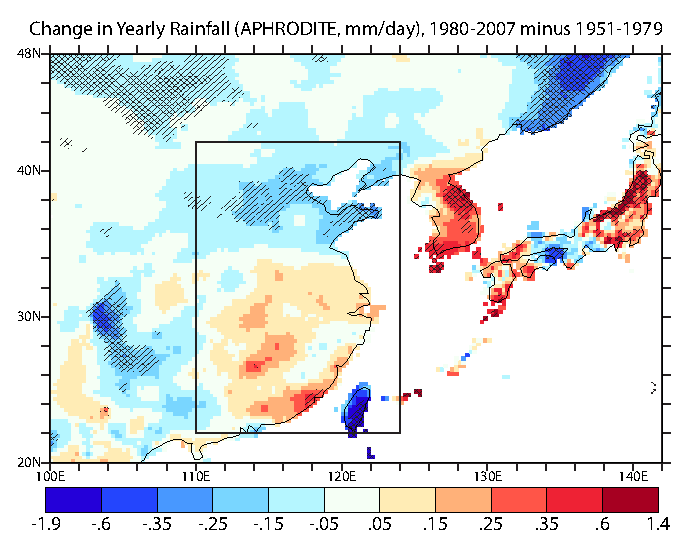
\includegraphics[width=36pc]{Figures/changes_2d_nojet}
\caption{Difference in yearly mean rainfall between 1980-2007 and 1951-1979. The South Flood-North Drought pattern is visible between 110-124$^{\circ}$E and 22-42$^{\circ}$N over mainland China (marked by box). Changes significant at a 95\%/99\% level are marked with single/double cross-hatches respectively.}
\label{fig:f31}
\end{figure}

\clearpage

%%EXPLANATORY FIGURES SHOWING ALGORITHM FUNCTIONALITY

%%FIGURE 3.2 - displaying continuous maximum criterion required to attempt rainband fit
\begin{figure}[htbp]
\centering
\noindent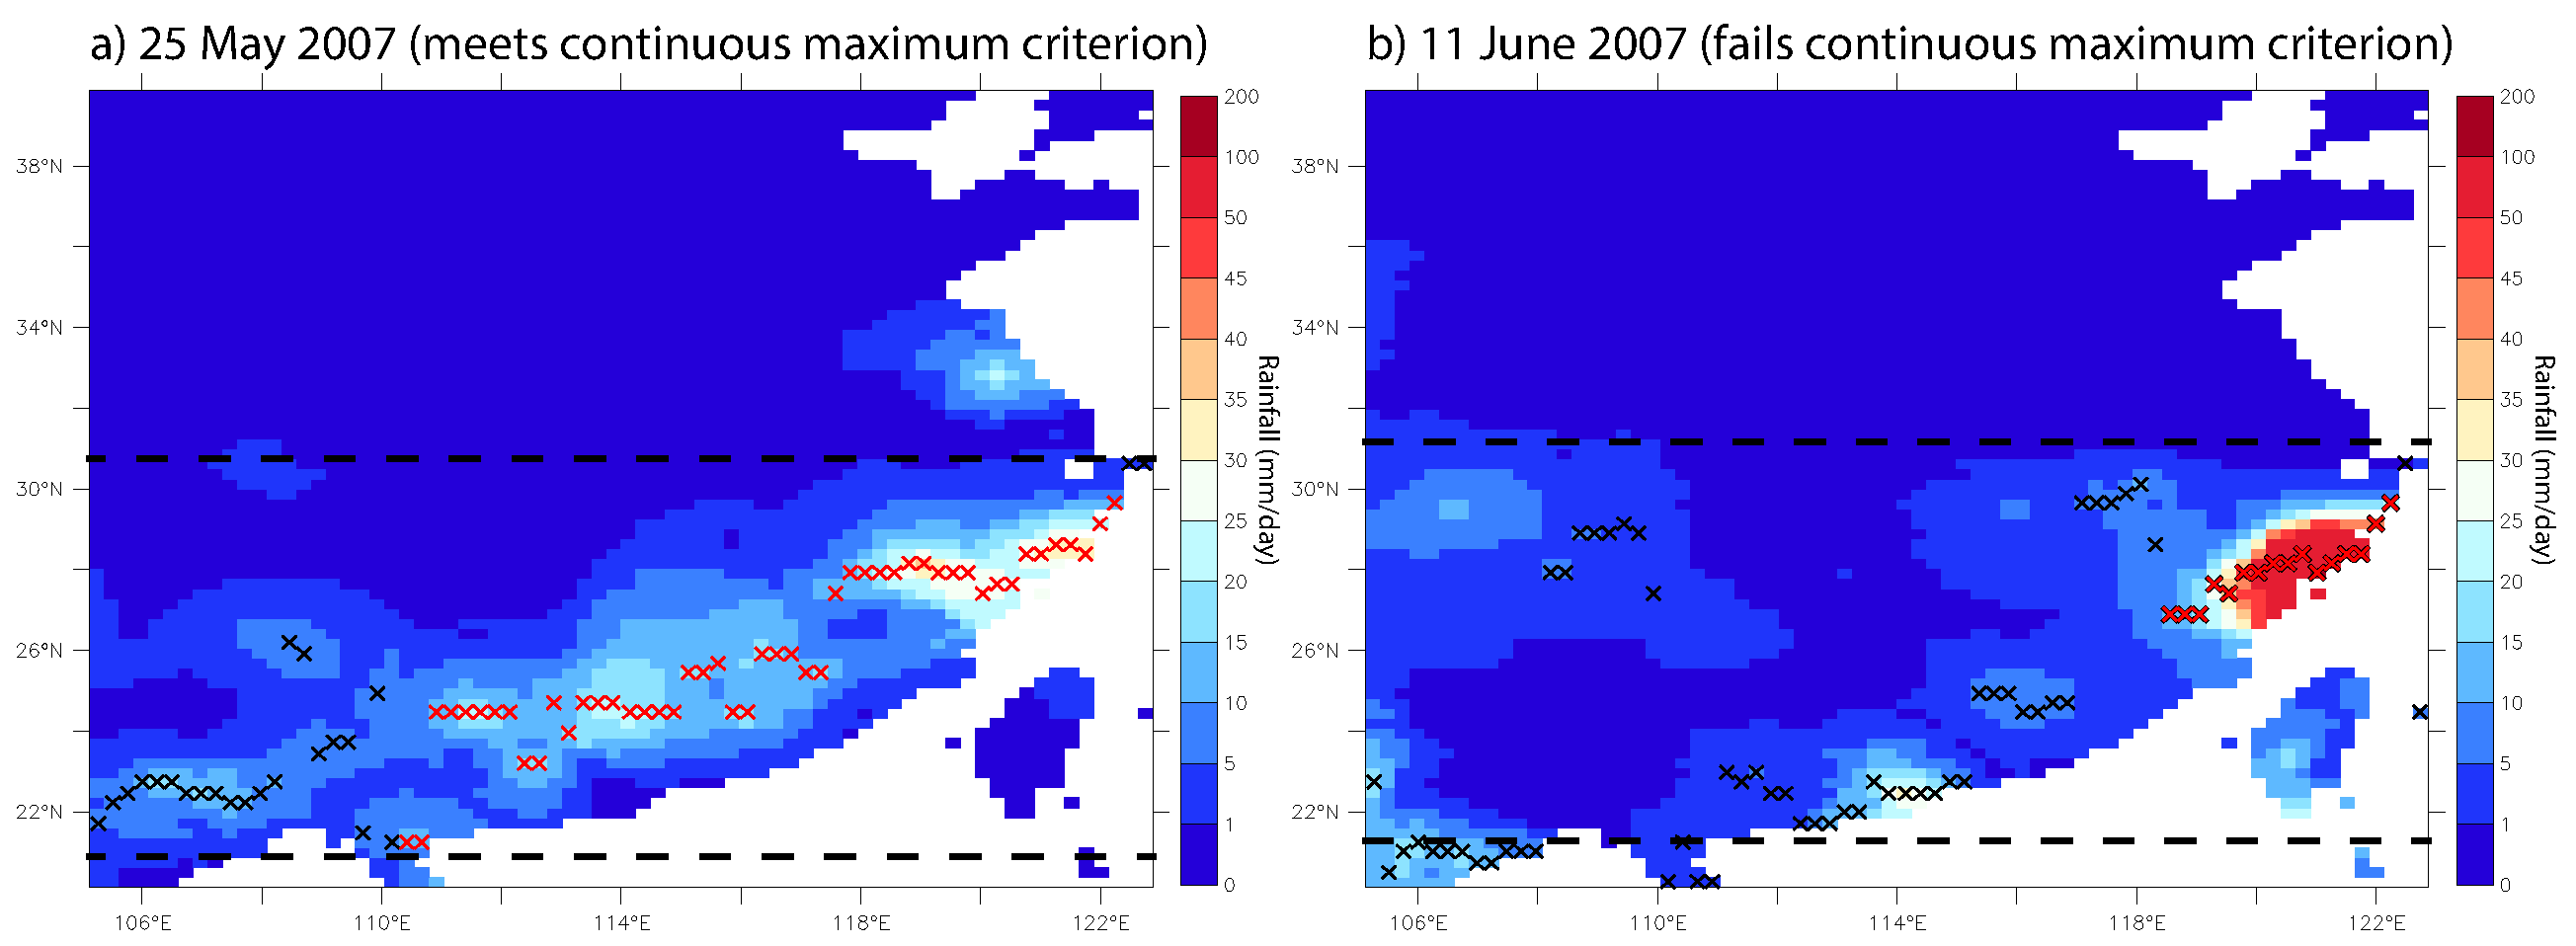
\includegraphics[width=40pc]{Figures/S1}
\caption{On each day, RDA first checks whether a continuous band of precipitation maxima exceeding 10 mm day$^{-1}$ exists that spans over 5 degrees of longitude. If so, a rainband fit is attempted. In panels a and b, the latitude of maximum precipitation at each longitude is marked with a black X. The longest continuous chain of maxima exceeding 10 mm day$^{-1}$ is marked in red. a) 25 May 2007 - the continuous maximum criterion is met and a fit is attempted.  b) 11 June 2007 - although there is abundant rainfall in some locations, no band is visible and the continuous maximum criterion is failed. No fit is attempted.}
\label{fig:f32}
\end{figure}

%%FIGURE 3.3 - How the convergent fit algorithm works.
\begin{figure}[htbp]
\centering
\noindent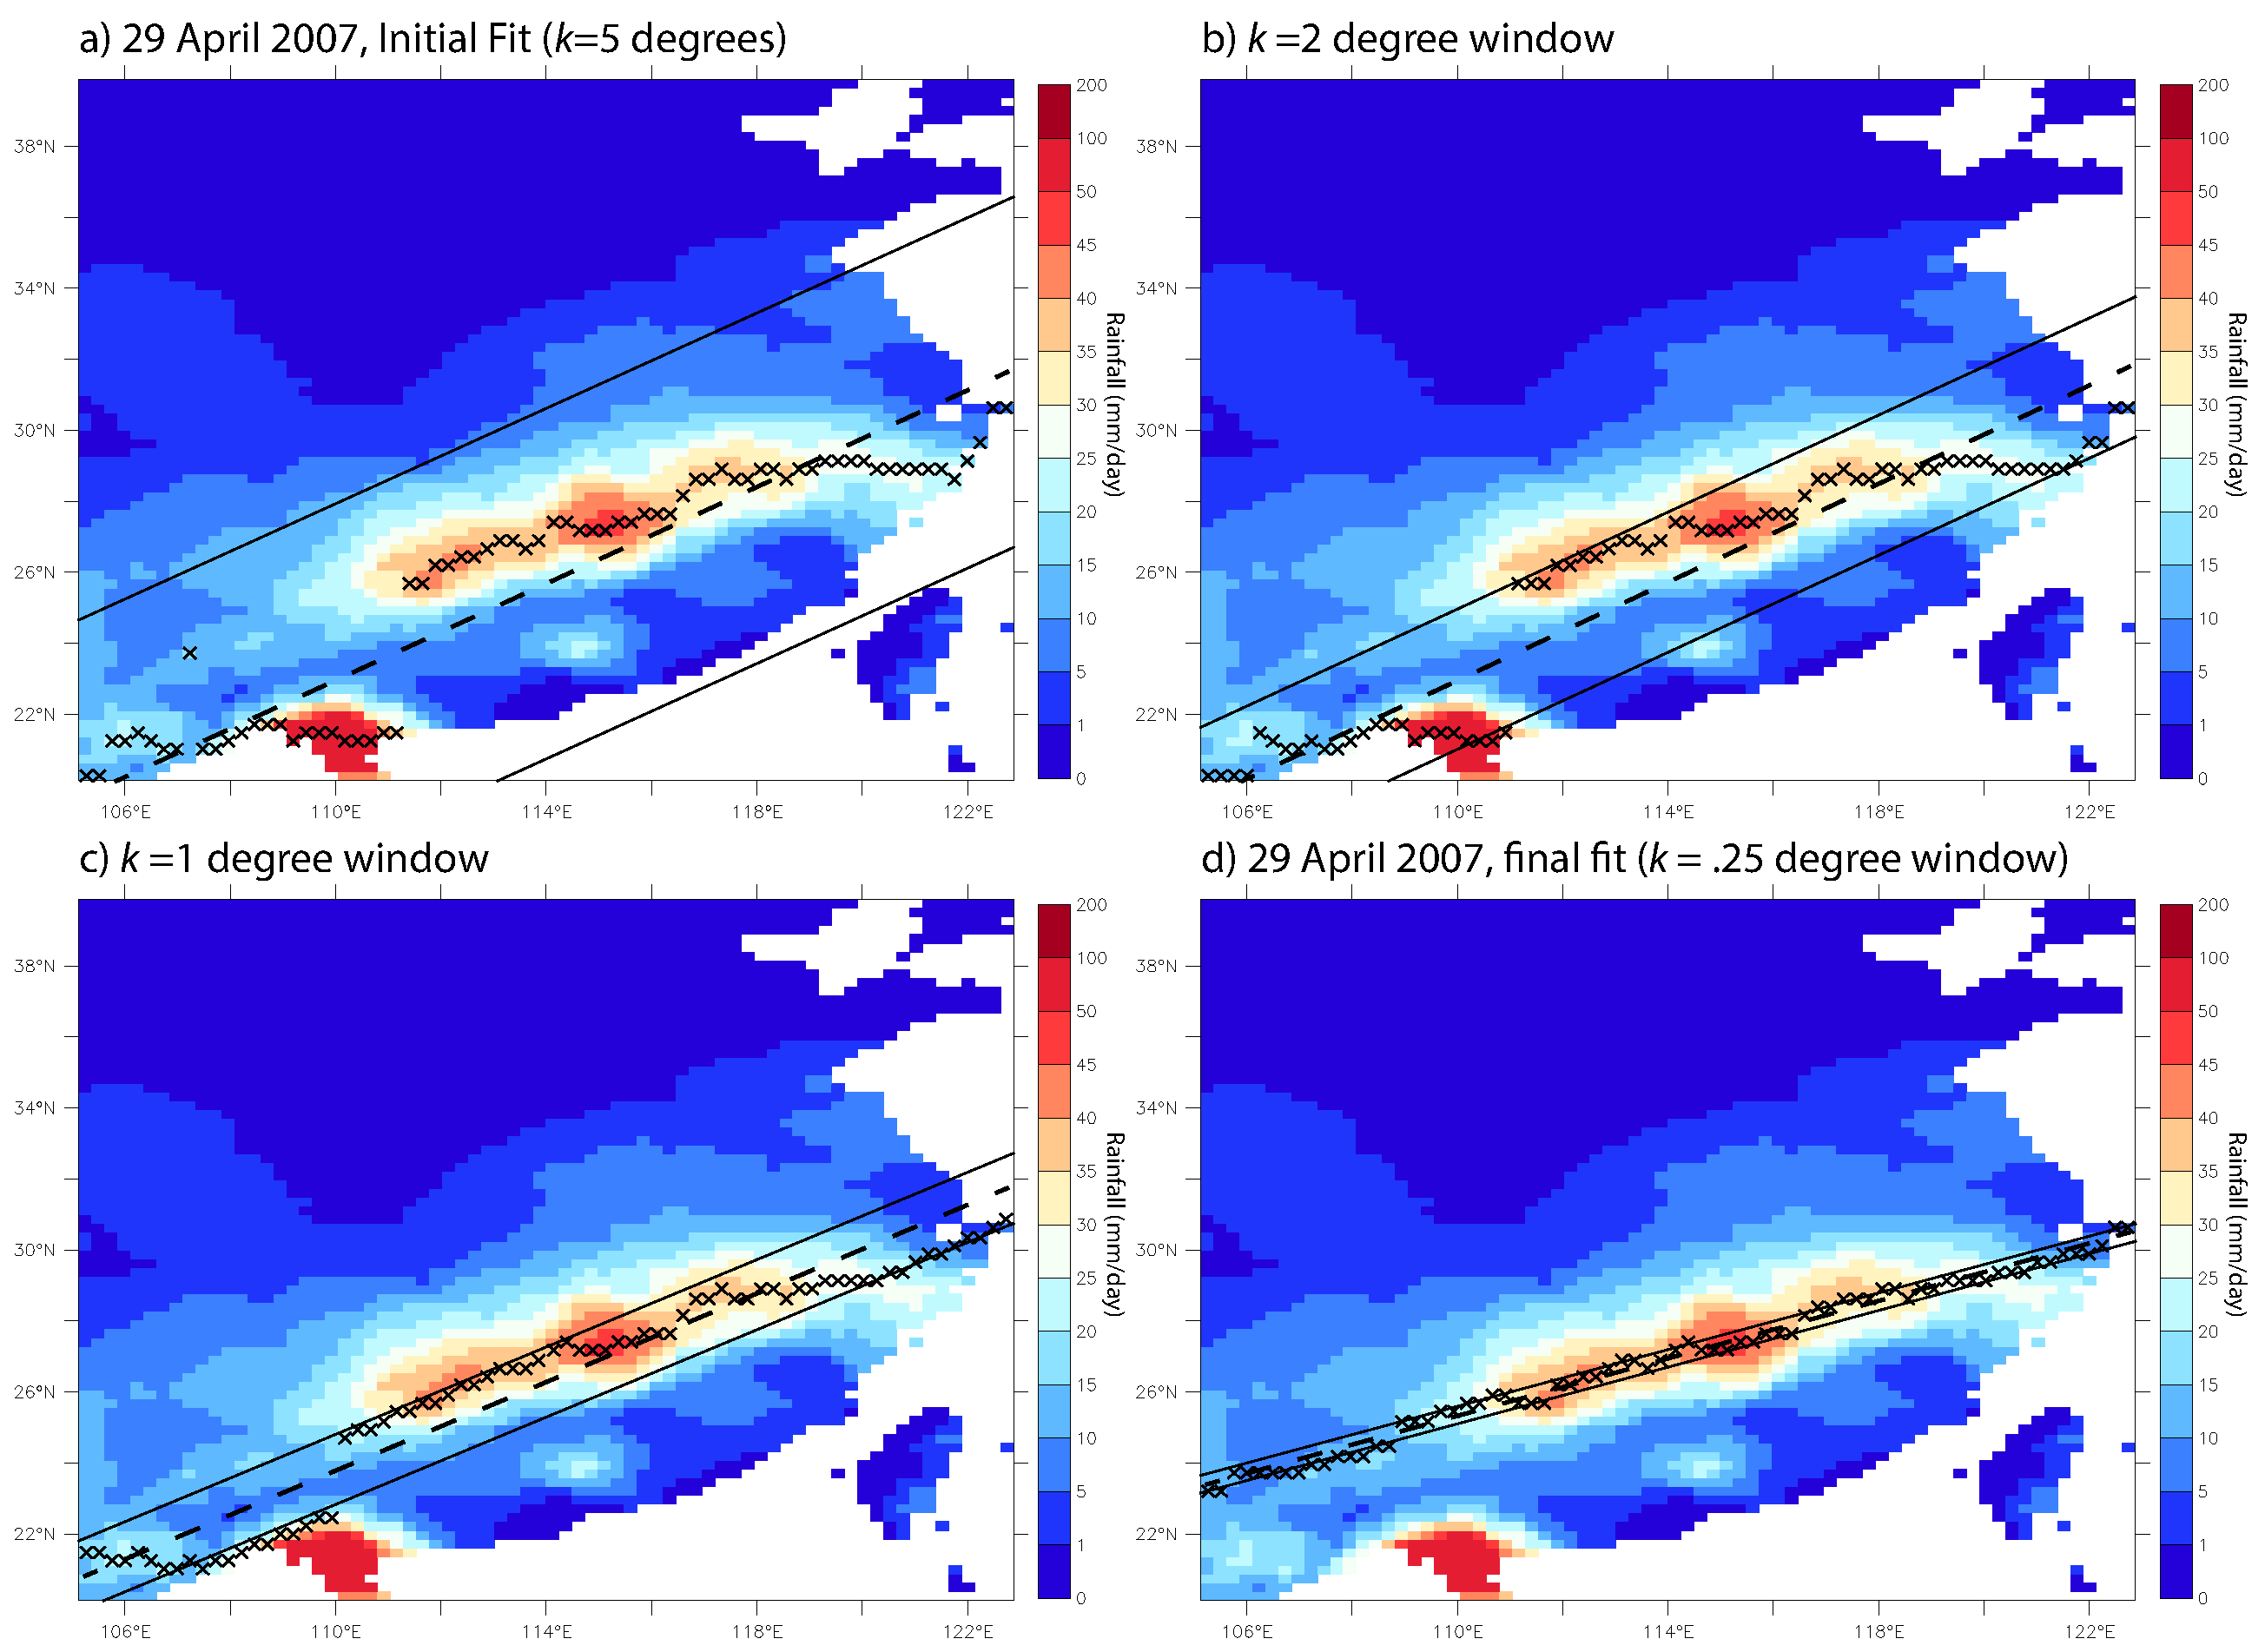
\includegraphics[width=40pc]{Figures/S2}
\caption{Display of the functionality of the recursive convergent fit. Dashed line shows estimated rainband position before each iteration and the solid lines indicate the window within we search for maxima. On 29 April 2007, a strong maximum in southernmost China skews our initial rainband fit (a), but the algorithm eventually converges on its true position via tighter windowing (d).}
\label{fig:f33}
\end{figure}

\clearpage

%%FIGURE 3.4 - Quality Control algorithm used to determine inclusion in statistics
\begin{figure}[htbp]
\centering
\noindent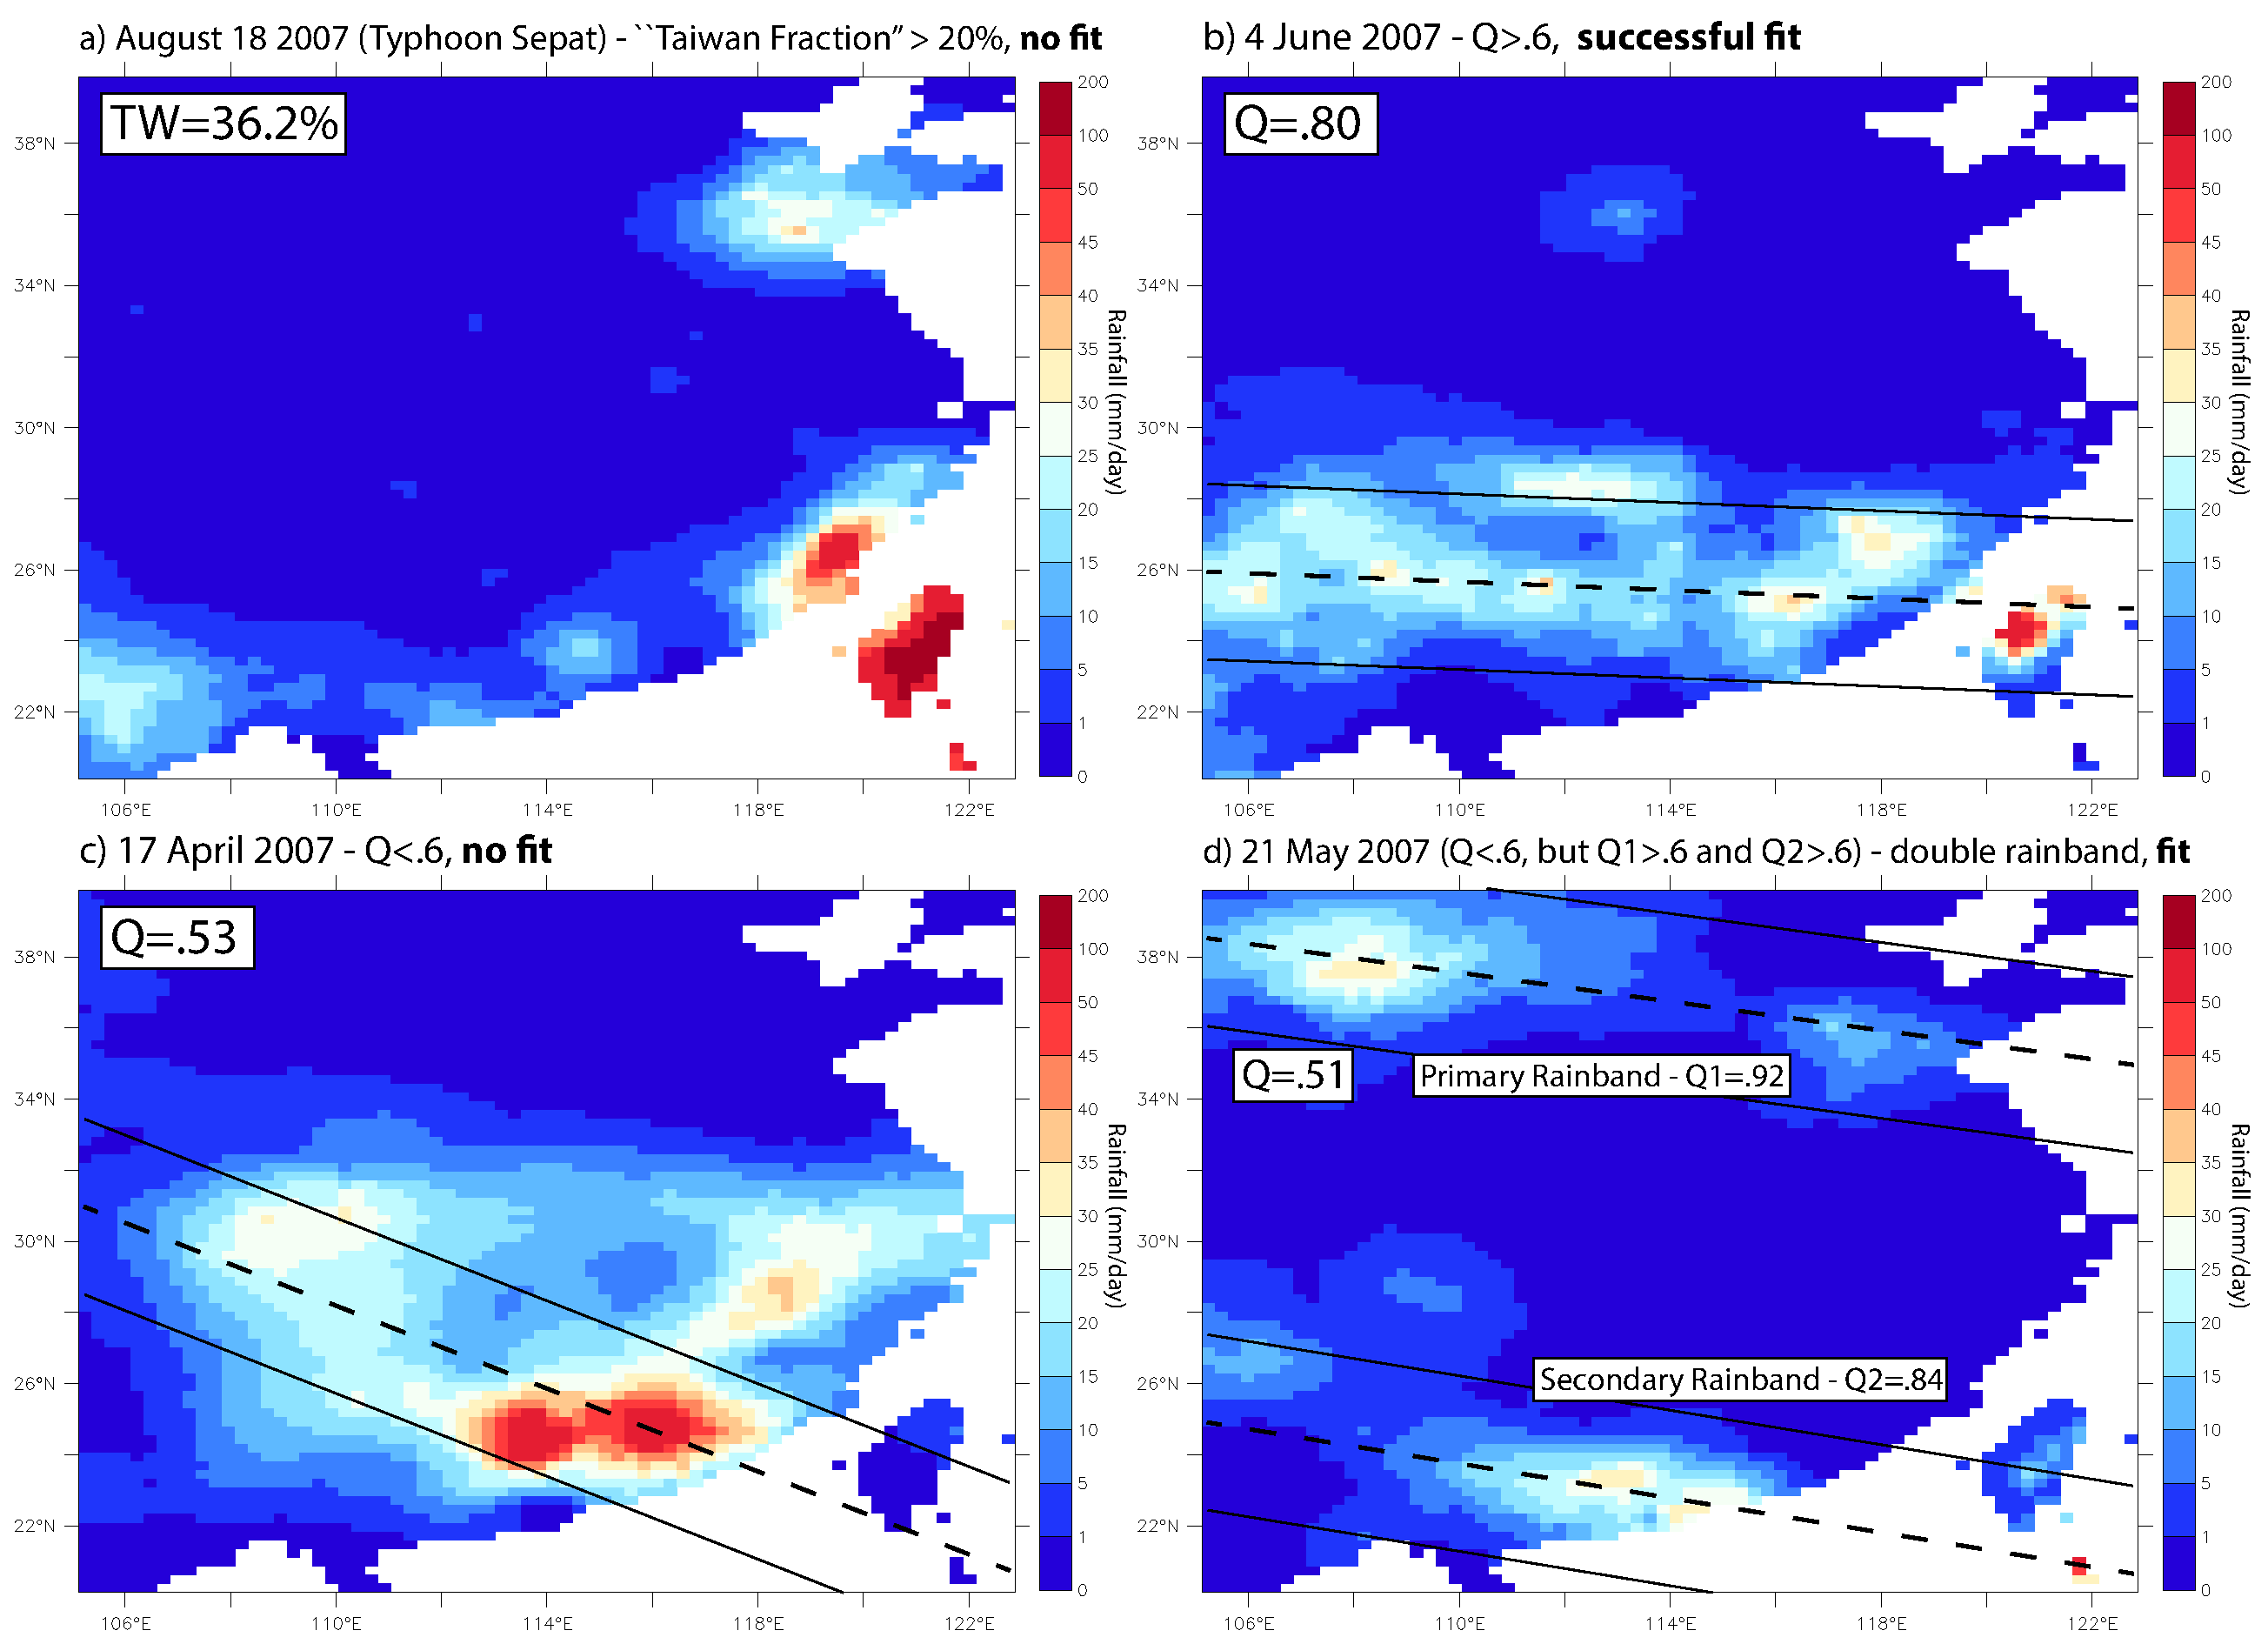
\includegraphics[width=40pc]{Figures/S4}
\caption{A quality control algorithm is used to exclude poor fits. a) 18 August 2007 - Days with a high Taiwan fraction (here, corresponding to the passage of Typhoon Sepat) are excluded from our statistics. b) June 4 2007 - A high-quality fit is achieved. c) 17 April 2007 - Although a tentative fit is obtained, it explains the distribution of rainfall poorly and is therefore unsuccessful. d) 21 May 2007 (same day as Figure~\ref{fig:f35}) - An initial fit appears to be of poor quality ($Q<.6$). However, after finding a secondary rainband, we determine that conditional quality scores $Q_1$ and $Q_2$ are sufficiently high, and the double rainband fit is successful.}
\label{fig:f34}
\end{figure}

%%FIGURE 3.5 - Procedure for finding double rainbands
\begin{figure}[htbp]
\centering
\noindent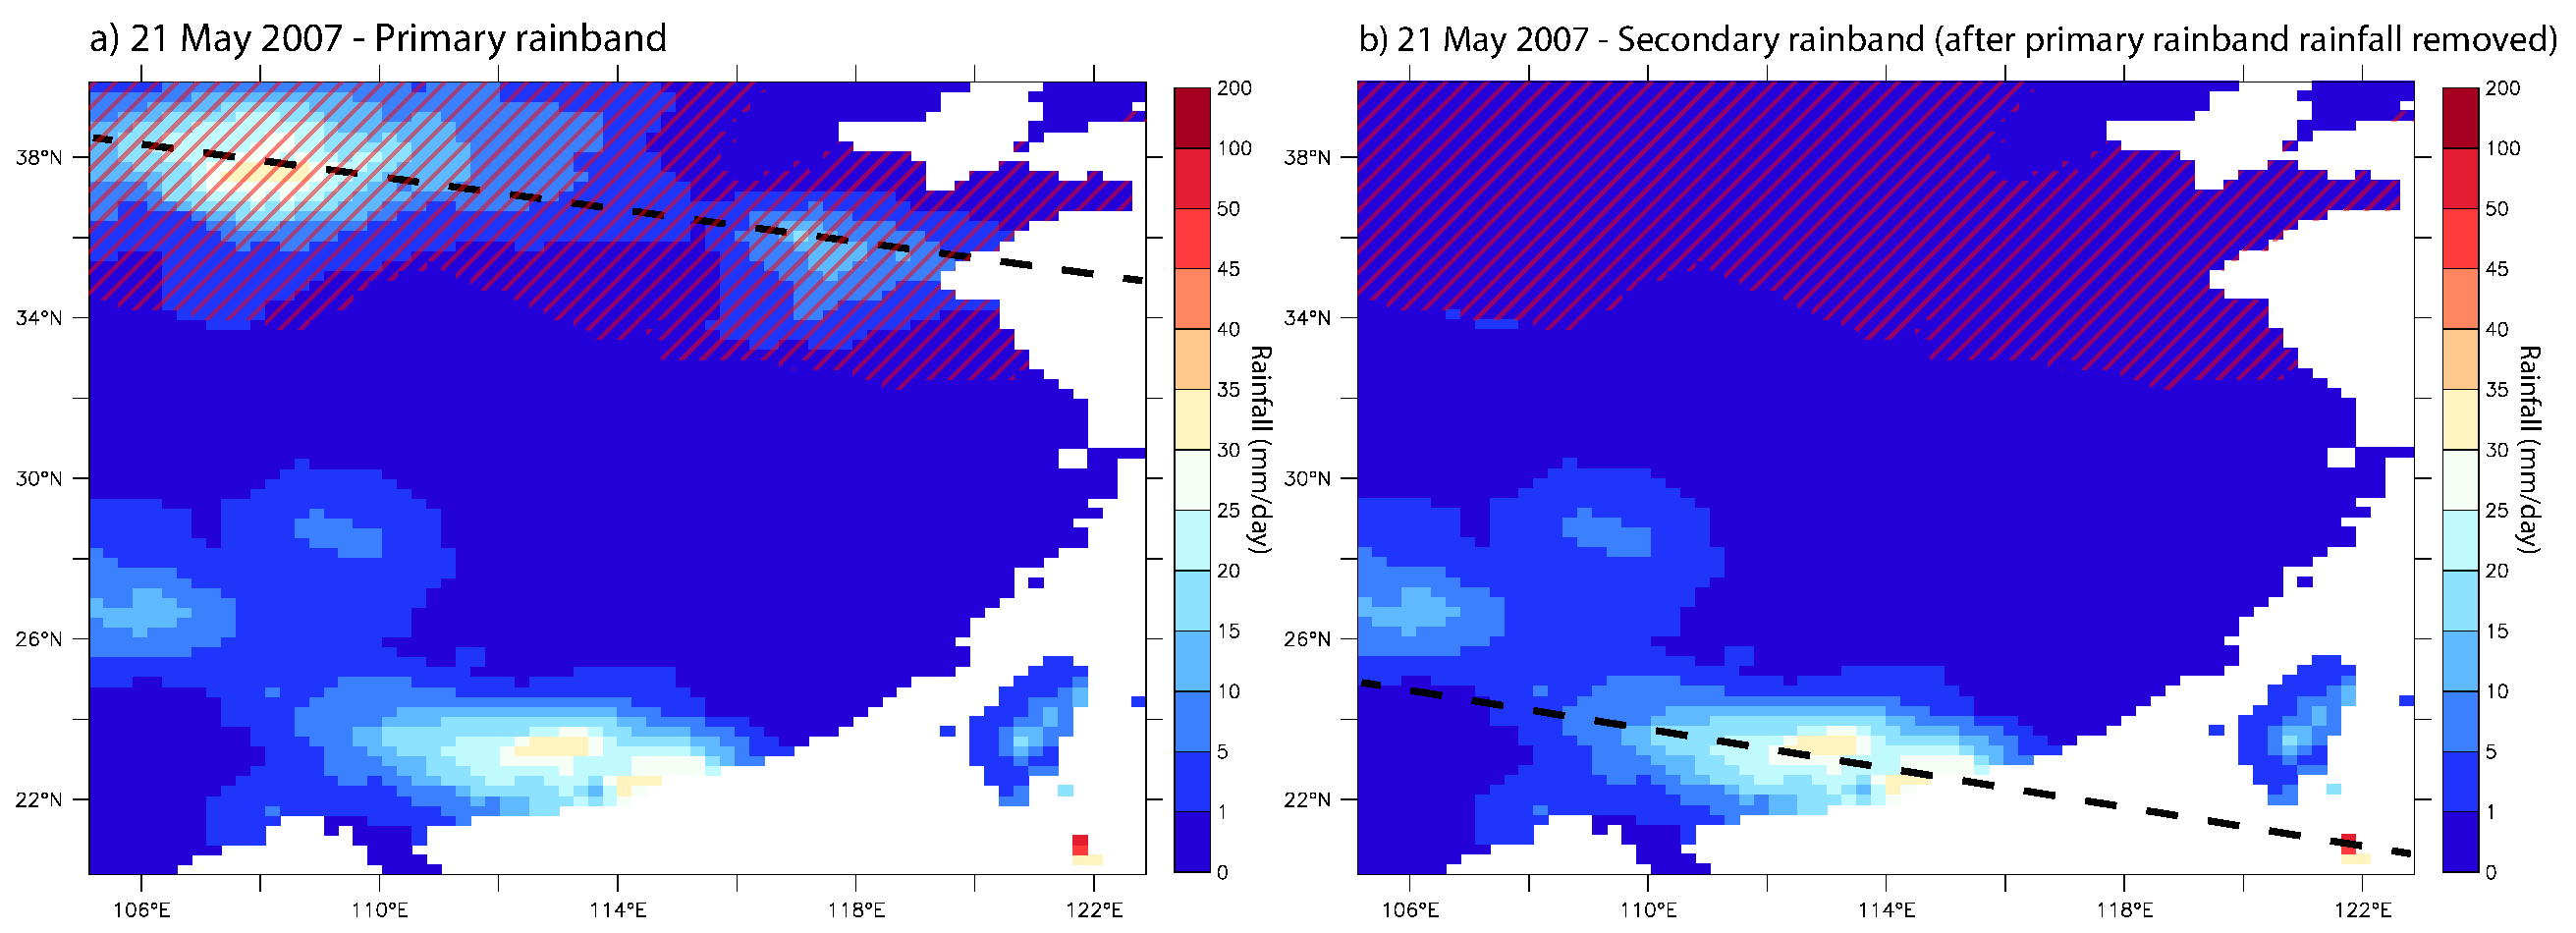
\includegraphics[width=42pc]{Figures/S3}
\caption{a) The first pass of the recursive fit algorithm converges on the strongest rainband, around 37$^{\circ}$N (defined as the ``primary rainband''). The \textit{banded rainfall} associated with the primary band is shaded with red hatchmarks. b) All banded rainfall from the primary band is removed, and we check for the presence of another rainband (a ``secondary rainband''), again using the continuous maximum criterion. When this criterion is satisfied, we find the secondary rainband's position with the recursive fit algorithm.}
\label{fig:f35}
\end{figure}

\clearpage

% FIGURES SHOWING RESULTS %%

%%FIGURE 3.6 Hovm�ller diagram of Meiyu latitude occupancy, 1951-2007. Produced by MATLAB scripts meiyufig1.m and meiyustats_compact.m.
\begin{figure}[htbp]
\centering
\noindent\includegraphics[width=32pc]{Figures/meiyu_hovmoller}
\caption{Climatology of East Asian rainfall and rainbands, 1951-2007, with important time periods marked as follows: 1 - Spring Rains; 2 - Pre-Meiyu; 3 - Meiyu; 4 - Post-Meiyu; 5 - Fall Rains. a) Hovm\"oller diagram of precipitation (100-123$^{\circ}$E longitudinal average); b) Hovm\"oller diagram of absolute probability of observing a rainband (both primary and secondary), smoothed in time with a 9-day and 2$^{\circ}$-running box filter; c) Probability of primary rainband occurrence and mean intensity (9-day running mean); d) The conditional probability of a secondary rainband given the presence of a primary rainband, as well as the mean tilt and length of primary rainband events (9-day running mean).}
\label{fig:hov}
\end{figure}

%%FIGURE 3.7 Percentage of total rainfall at each point that is delivered through rainbands
\begin{figure}[htb]
\centering
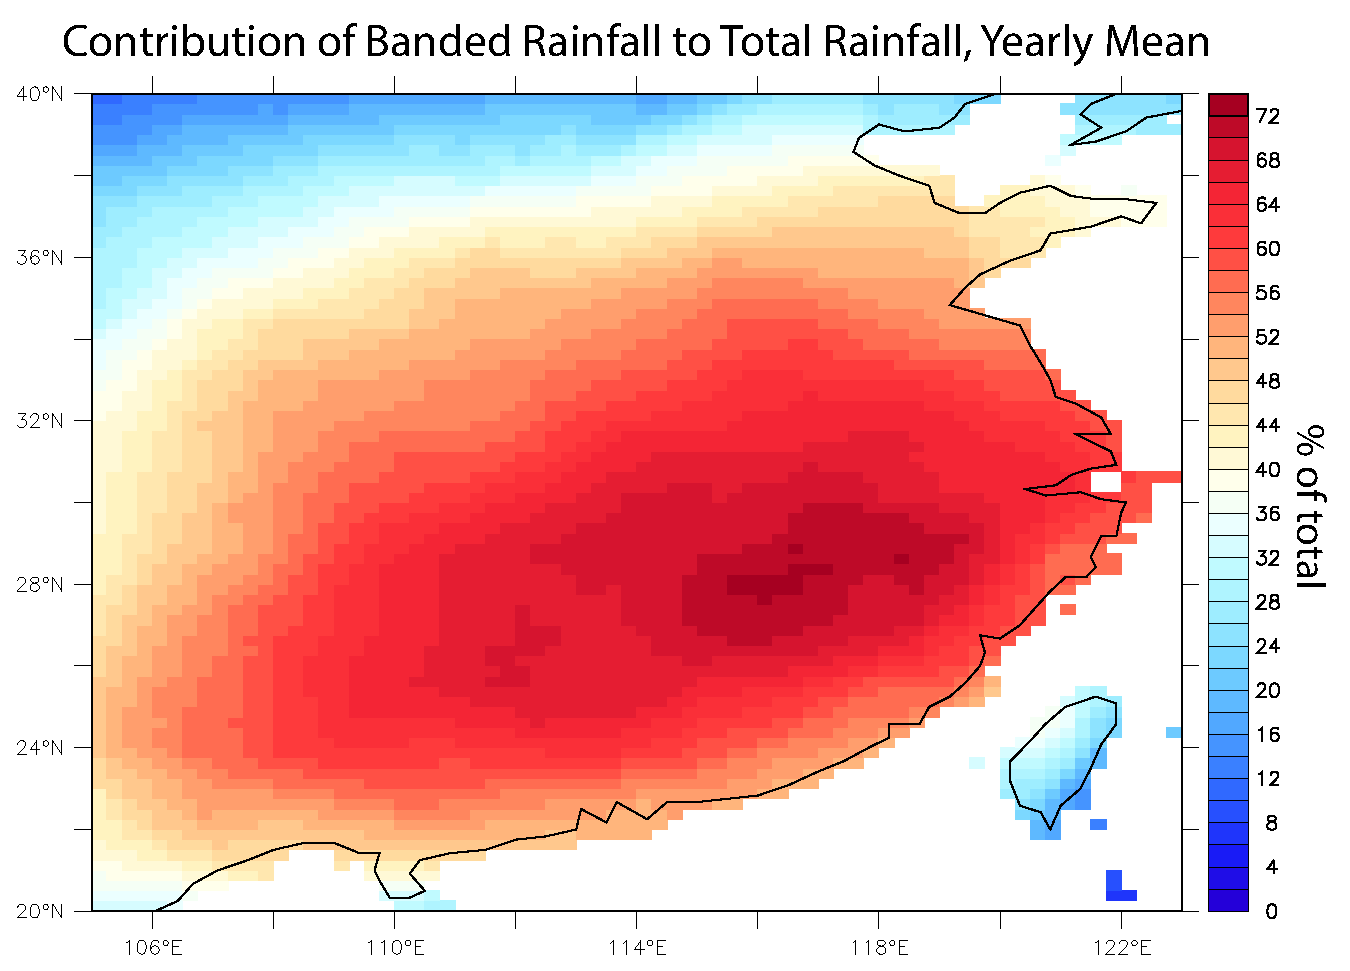
\includegraphics[width=36pc]{Figures/frontpct}
\caption{Yearly mean percentage of total rainfall that falls as banded rainfall. On a given day, banded rainfall consists of all rainfall falling within 4$^{\circ}$ of a rainband axis and rainfall at any other adjacent point exceeding 10 mm day$^{-1}$.}
\label{fig:frontpct}
\end{figure}

%%FIGURE 3.8 Changes in Meiyu and rainfall behavior between 1951-1979 and 1980-2007
\begin{figure}[htbp]
\centering
\noindent\includegraphics[width=36pc]{Figures/changes}
\caption{a) 15-day running mean of the change in rainfall between 1951-1979 and 1980-07, with 95\%/99\% confidence level marked by single/double cross-hatches; b) 15-day running mean of the change in rainband frequency between 1951-1979 and 1980-07, with two-degree smoothing in latitude and confidence levels marked as in a). The significance of rainfall changes is calculated by a permutation method. Time periods are marked as in Figure~\ref{fig:hov}: 1 - Spring Rains; 2 - Pre-Meiyu; 3 - Meiyu; 4 - Post-Meiyu; 5 - Fall Rains.}
\label{fig:changes}
\end{figure}

%%FIGURE 3.9 Climatology of alternative metrics of China rainfall
\begin{figure}[htb]
\centering
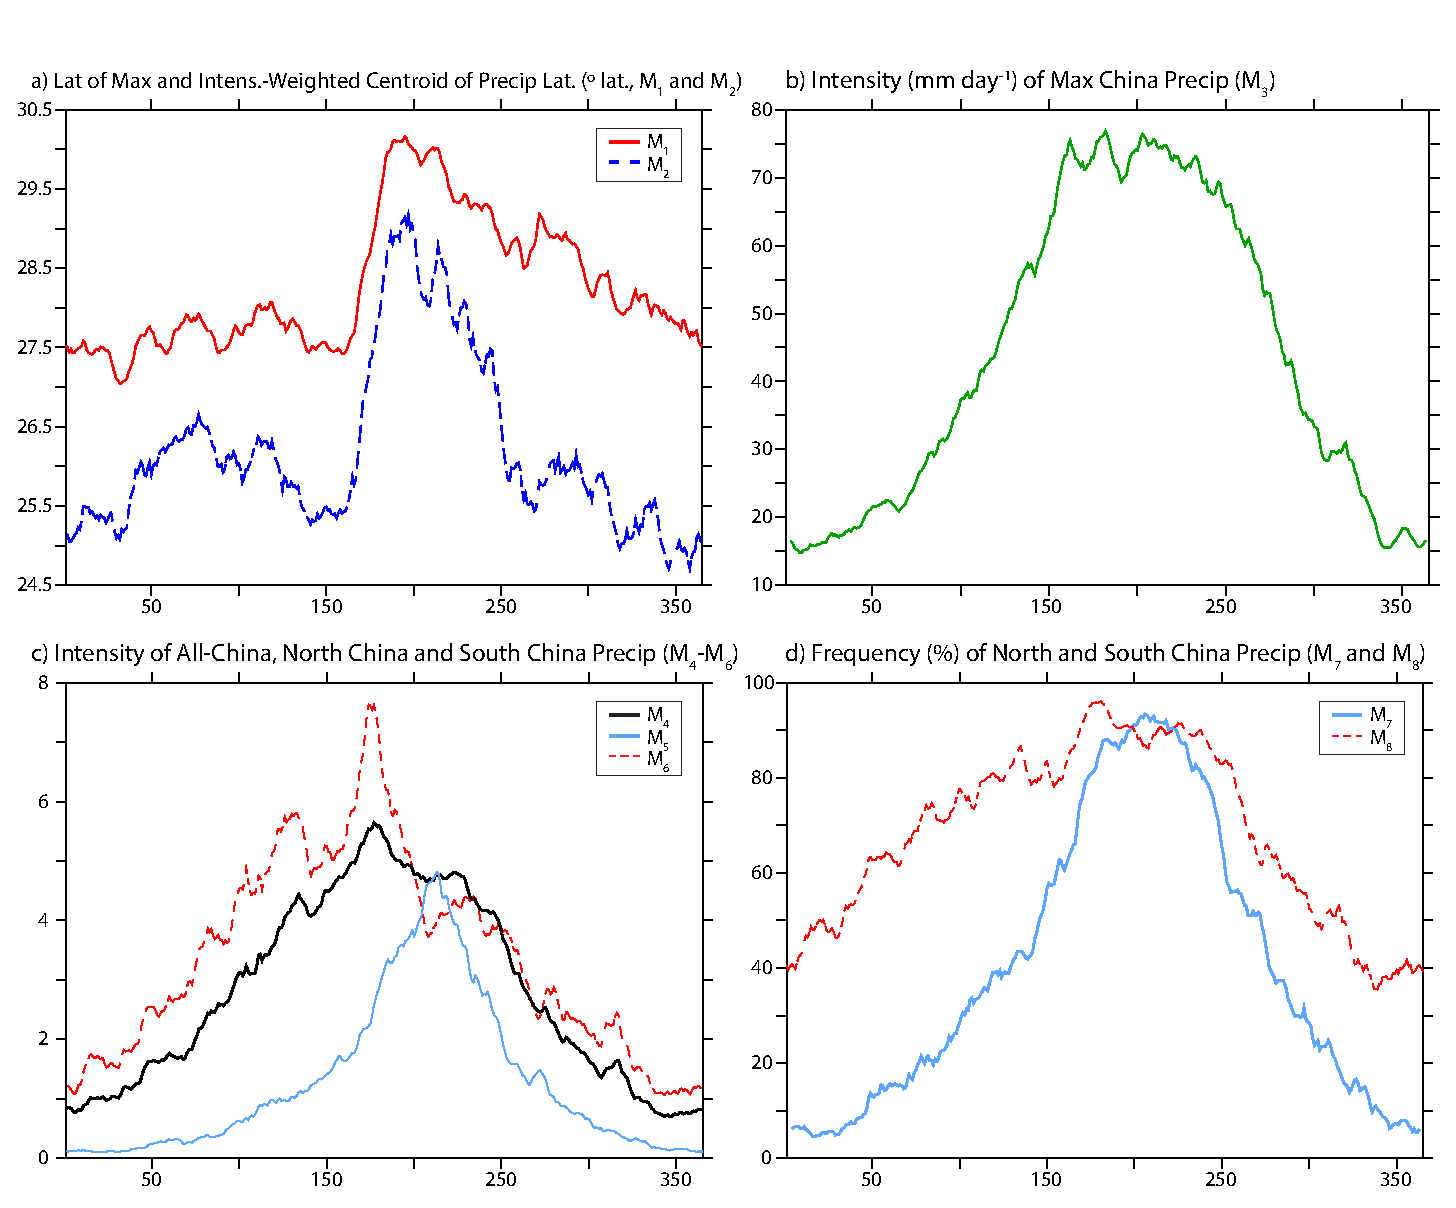
\includegraphics[width=36pc]{Figures/met_climo}
\caption{Yearly climatology of alternative metrics of China rainfall $M_1-M_8$. a) Latitude of maximum precipitation (blue dash, $M_1$) and intensity-weighted centroid of precipitation latitude (red, $M_2$); b) Intensity of maximum precipitation over China ($M_3$); c) Mean intensity of China rainfall (black, $M_4$), North China rainfall (thin light blue, $M_5$) and South China rainfall (red dash, $M_6$); d) Frequency of North China rainfall (light blue, $M_7$) and South China rainfall (red, $M_8$). China region is defined as 105-123$^{\circ}$E and 20-40$^{\circ}$N, North China as 107.5-125$^{\circ}$E and 37-42$^{\circ}$N and South China as 107.5-122.5$^{\circ}$E and 27-33$^{\circ}$N.}
\label{fig:type_changes}
\end{figure}

%%FIGURE 3.10 Decadal changes in different rainfall types
%potential change - add the total change in rainfall for each of the time periods (third column of panels)
\begin{figure}[htb]
\centering
\noindent\includegraphics[width=36pc]{Figures/decadal_front}
\caption{1980-2007 versus 1951-1979 changes in banded and local rainfall for full year (a and b respectively), Pre-Meiyu (c and d) and Post-Meiyu (e and f), with significance at the 95\%/99\% level marked by single/double hatches.  On a given day, \textit{banded} rainfall consists of all rainfall falling within 4$^{\circ}$ of a rainband axis and rainfall at any other adjacent point exceeding 10 mm day$^{-1}$. \textit{Local} rainfall includes all other rainfall.}
\label{fig:decadal_front}
\end{figure}

\end{document}